\documentclass[a4paper]{ltjsarticle}

\usepackage[margin=15mm]{geometry}

\usepackage{graphicx}
\usepackage{makeidx}
\usepackage[font=current]{idxlayout}
\makeindex

\begin{document}

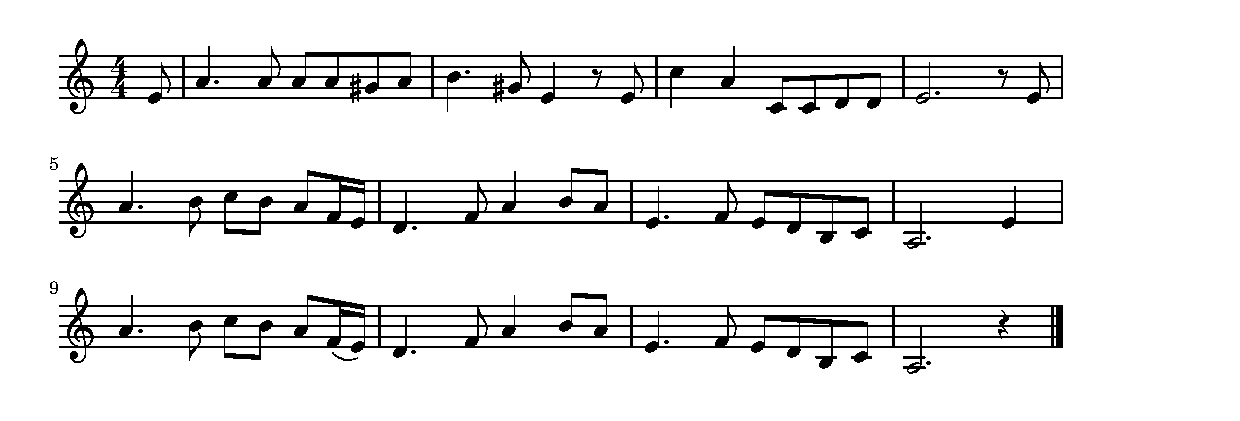
\includegraphics[clip]{troika_crop.pdf}

\vspace{-10mm} \hspace{10mm}
トロイカ(ゆきのしらかばなみき)
\index{とろいか@トロイカ(ゆきのしらかばなみき)}

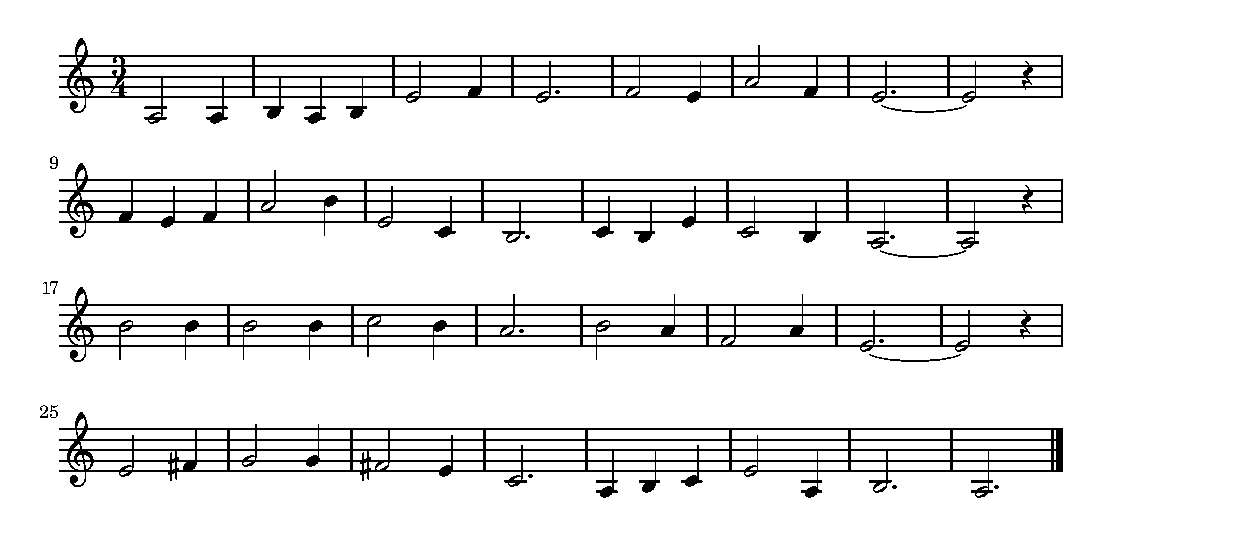
\includegraphics[clip]{utsukushiki_crop.pdf}

\vspace{-10mm} \hspace{10mm}
美しき天然(そらにさえずるとりのこえ)
\index{うつくしき@美しき天然(そらにさえずるとりのこえ)}

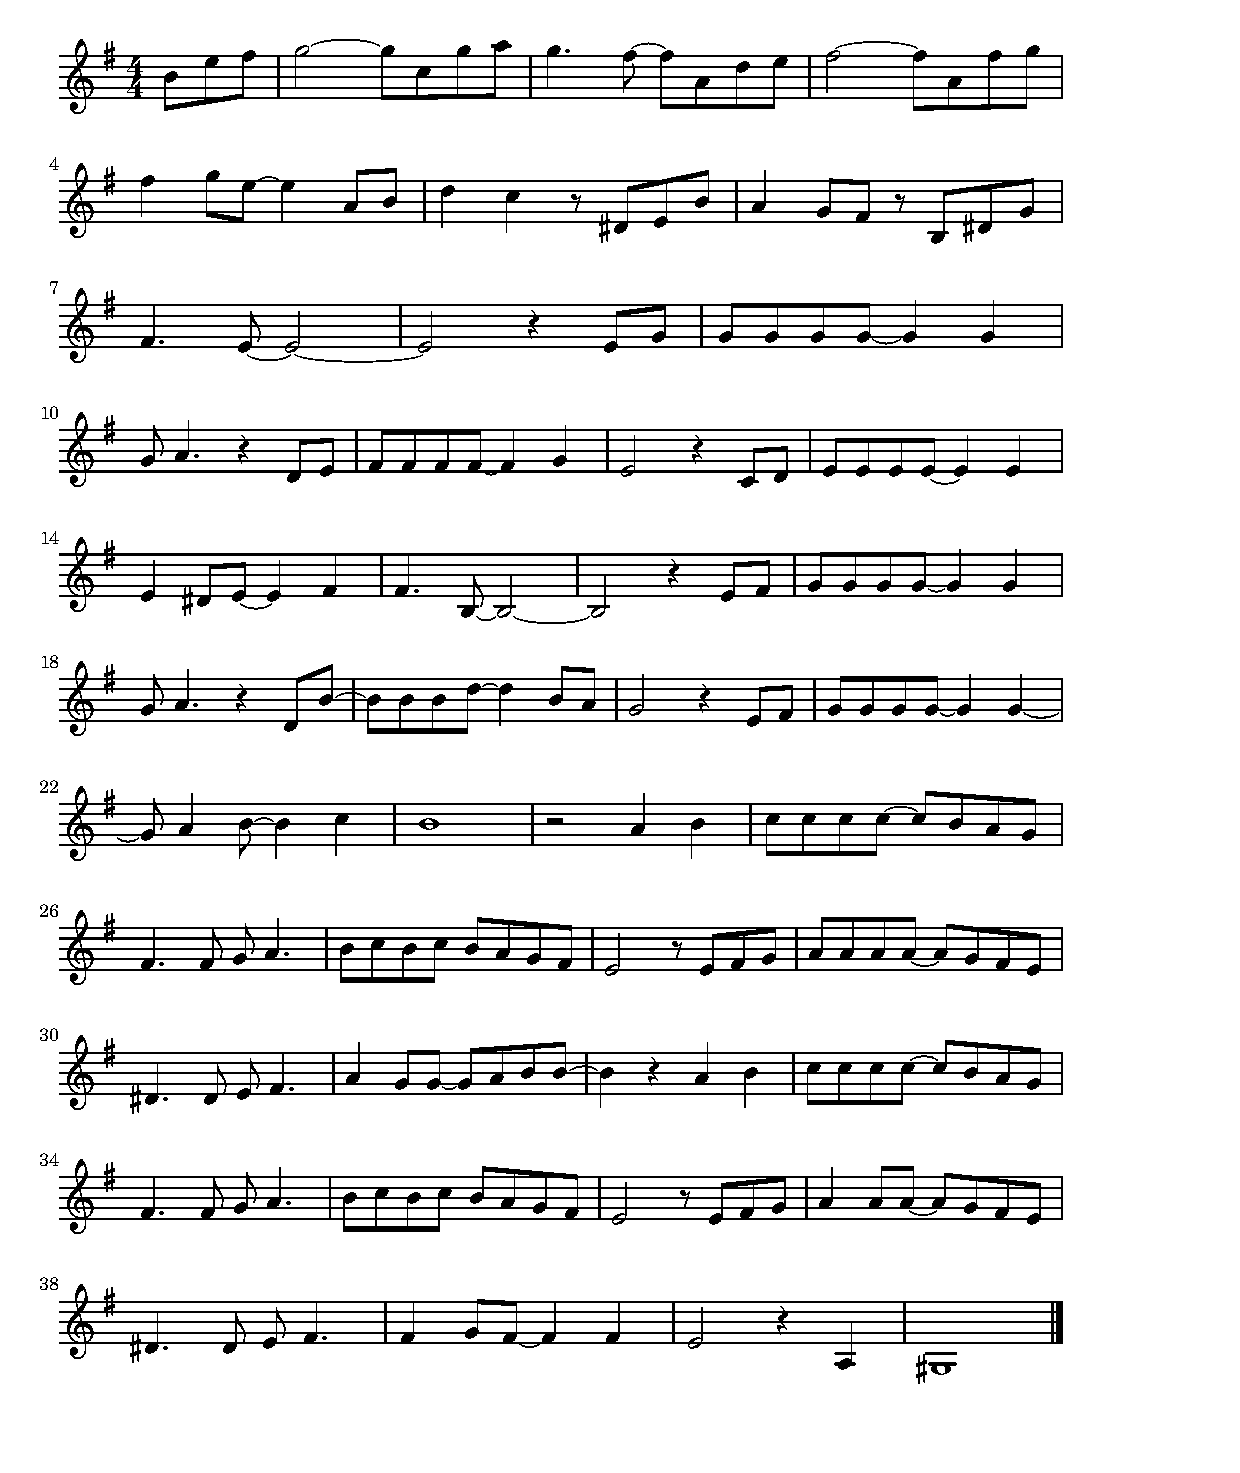
\includegraphics[clip]{fuyunosonata_crop.pdf}

\vspace{-10mm} \hspace{10mm}
冬のソナタ(最初から今まで )
\index{ふゆのそなた@冬のソナタ(最初から今まで)}
\index{さいしょから@冬のソナタ(最初から今まで)}

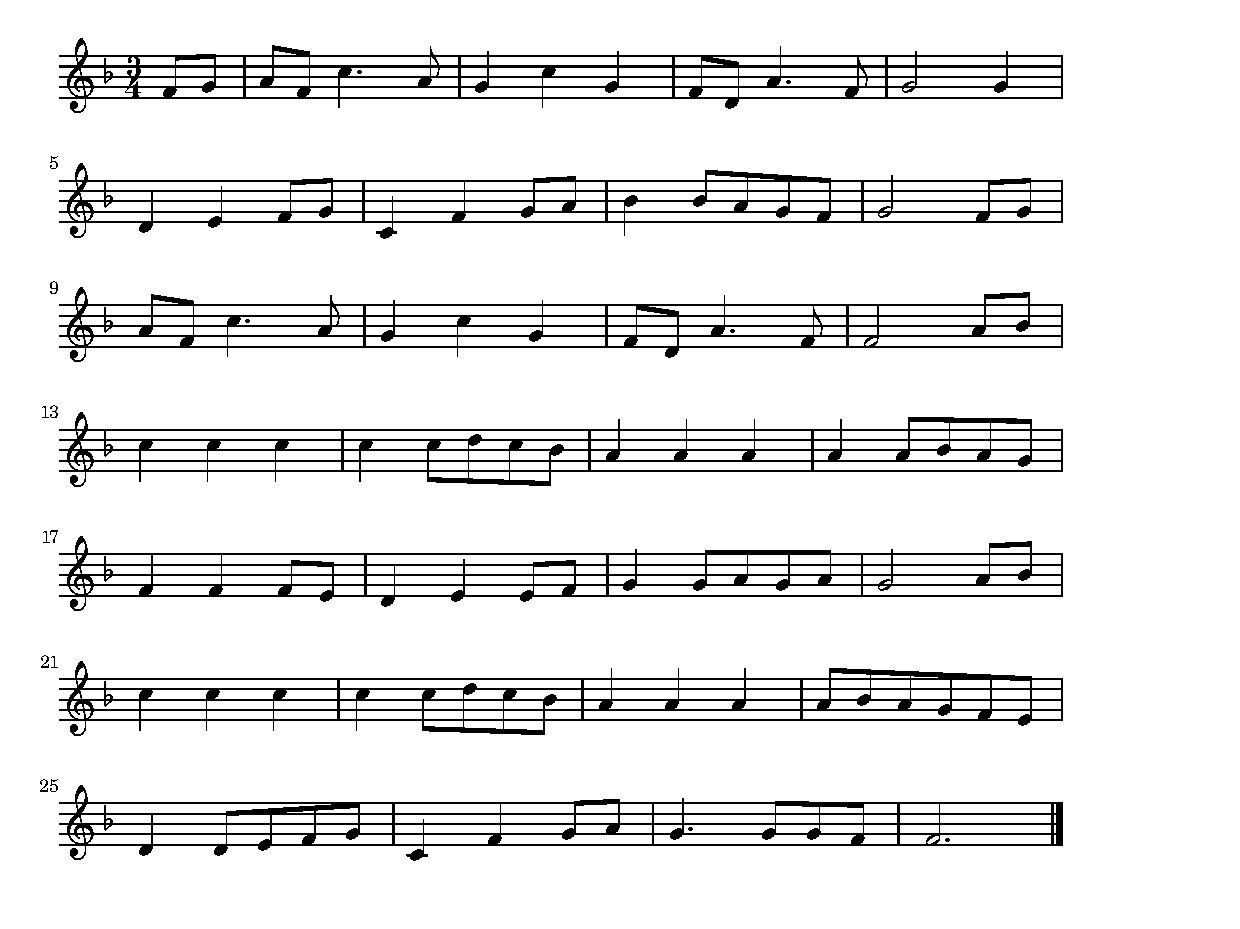
\includegraphics[clip]{itsumonando_crop.pdf}

\vspace{-10mm} \hspace{10mm}
いつも何度でも(千と千尋の神隠し。よんでいるどこかむねのおくで)
\index{いつも@いつも何度でも(千と千尋の神隠し。よんでいるどこかむねのおくで)}

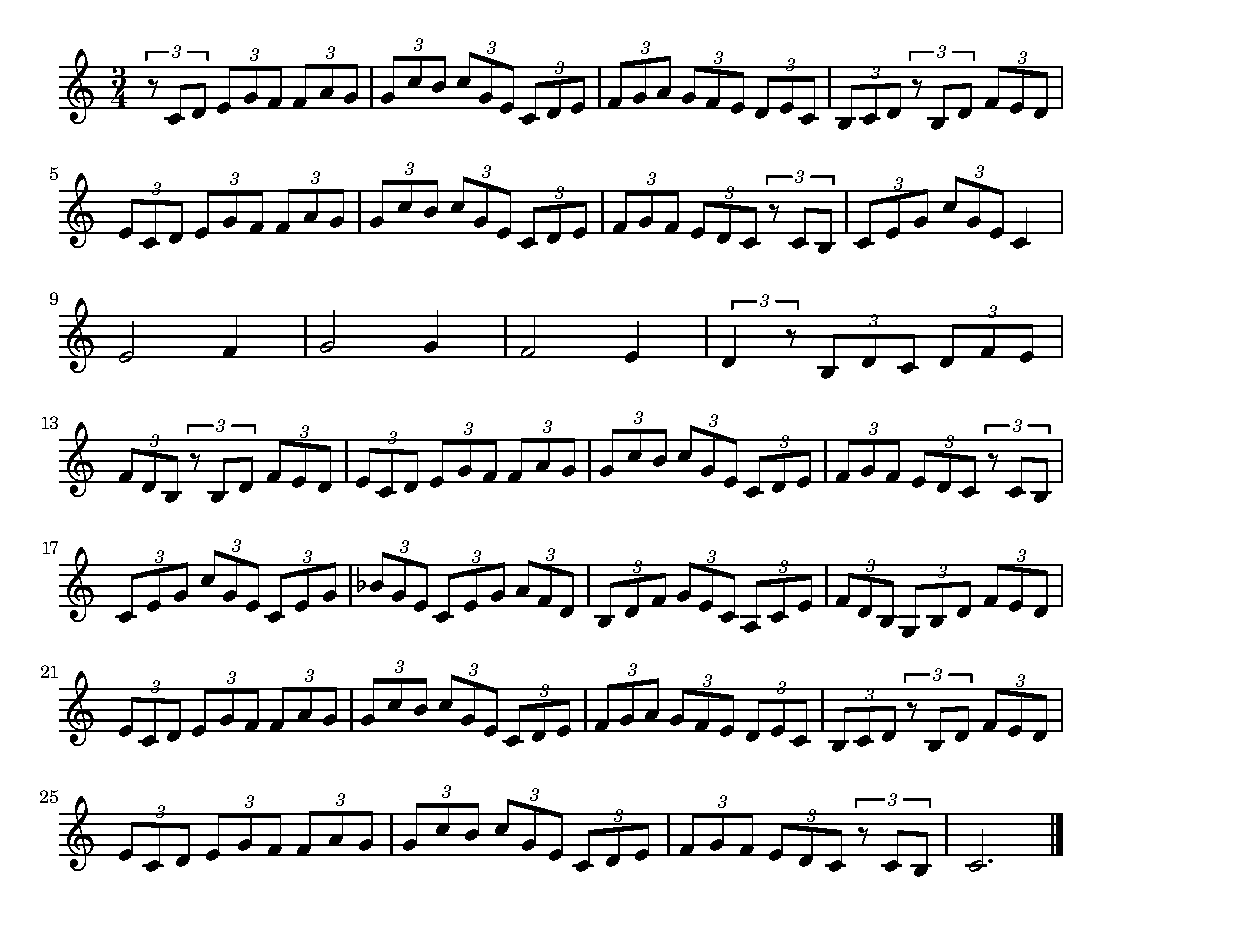
\includegraphics[clip]{shuyohitononozomino_crop.pdf}

\vspace{-10mm} \hspace{10mm}
主よ人の望みの喜びよ(J.S.バッハ)
\index{しゅよ@主よ人の望みの喜びよ(J.S.バッハ)}
\index{ばっは@主よ人の望みの喜びよ(J.S.バッハ)}

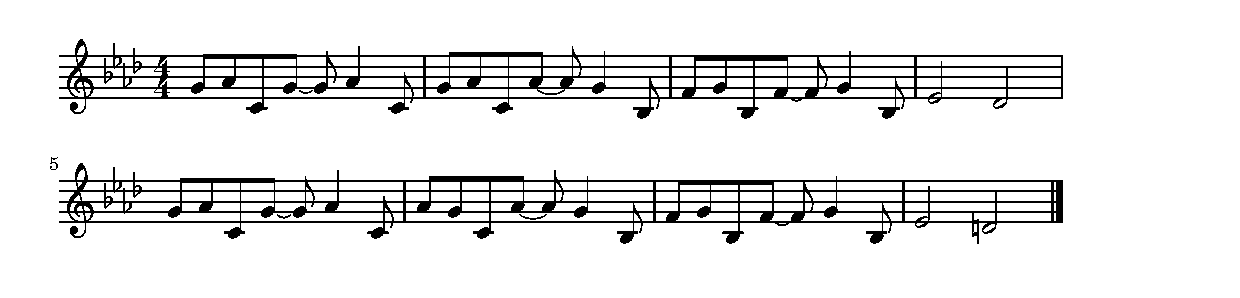
\includegraphics[clip]{letitgointro_crop.pdf}

\vspace{-10mm} \hspace{10mm}
ありのままで(アナと雪の女王イントロ。let It Go)
\index{ありのままで@ありのままで(アナと雪の女王イントロ。let It Go)}

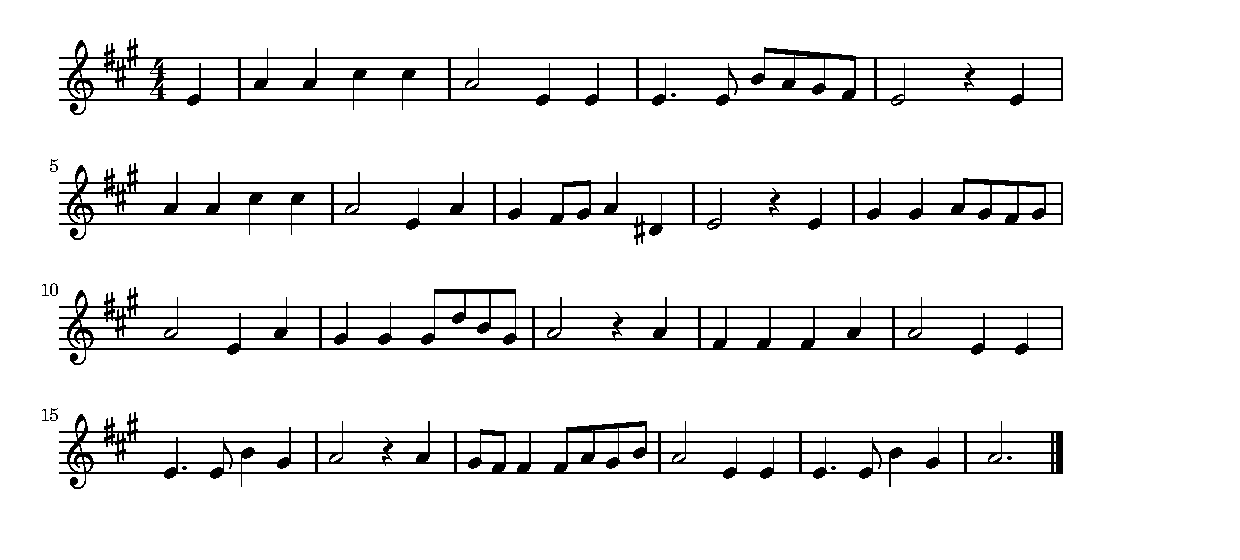
\includegraphics[clip]{masu_crop.pdf}

\vspace{-10mm} \hspace{10mm}
ます(シューベルト)
\index{ます@ます(シューベルト)}
\index{しゅーべると@ます(シューベルト)}

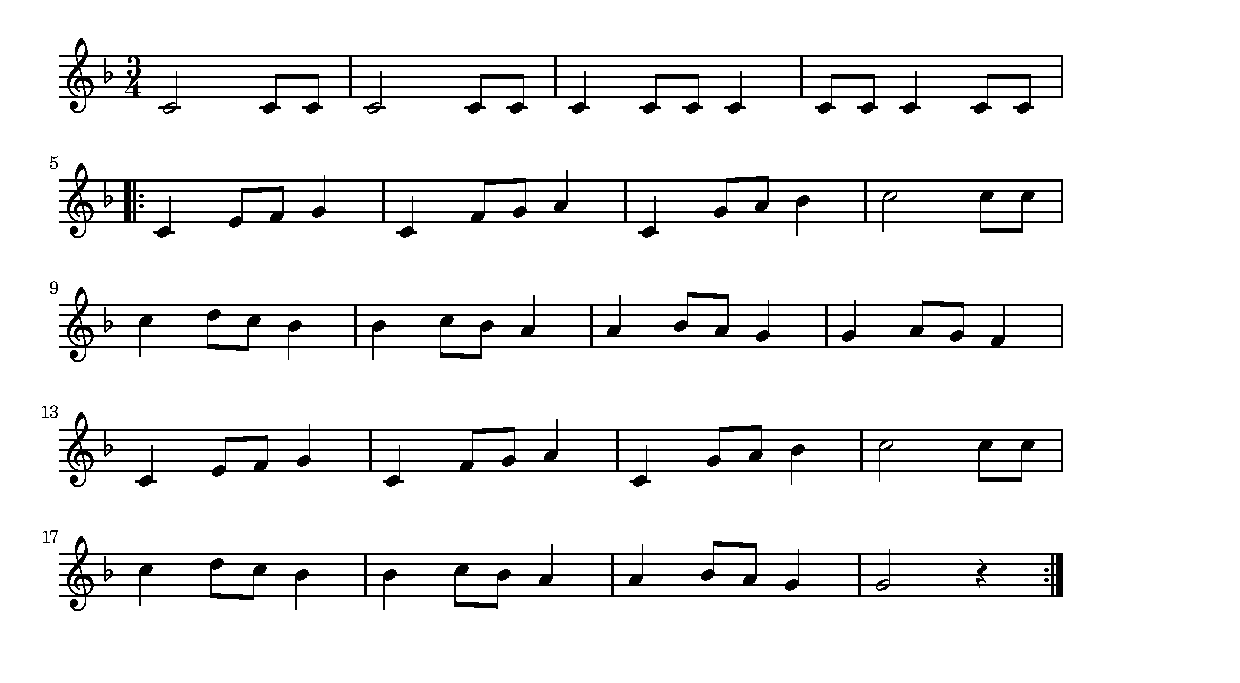
\includegraphics[clip]{kareinaru_crop.pdf}

\vspace{-10mm} \hspace{10mm}
華麗なる大円舞曲(ショパン)
\index{かれいなる@華麗なる大円舞曲(ショパン)}
\index{しょぱん@華麗なる大円舞曲(ショパン)}

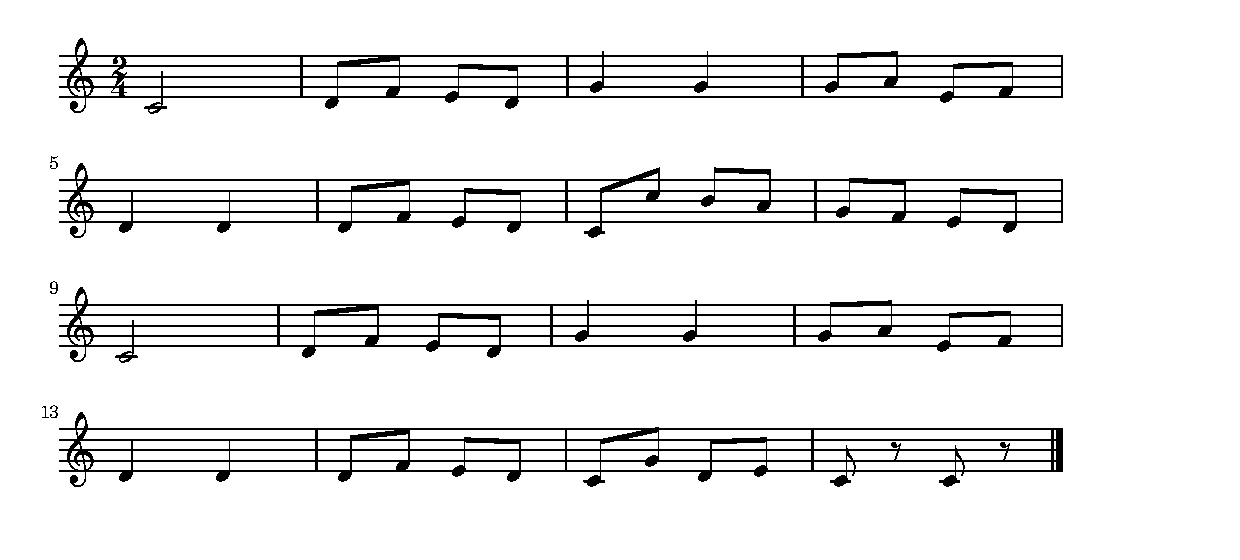
\includegraphics[clip]{tengokujigoku_crop.pdf}

\vspace{-10mm} \hspace{10mm}
天国と地獄(オッフェンバック)
\index{てんごく@天国と地獄(オッフェンバック)}

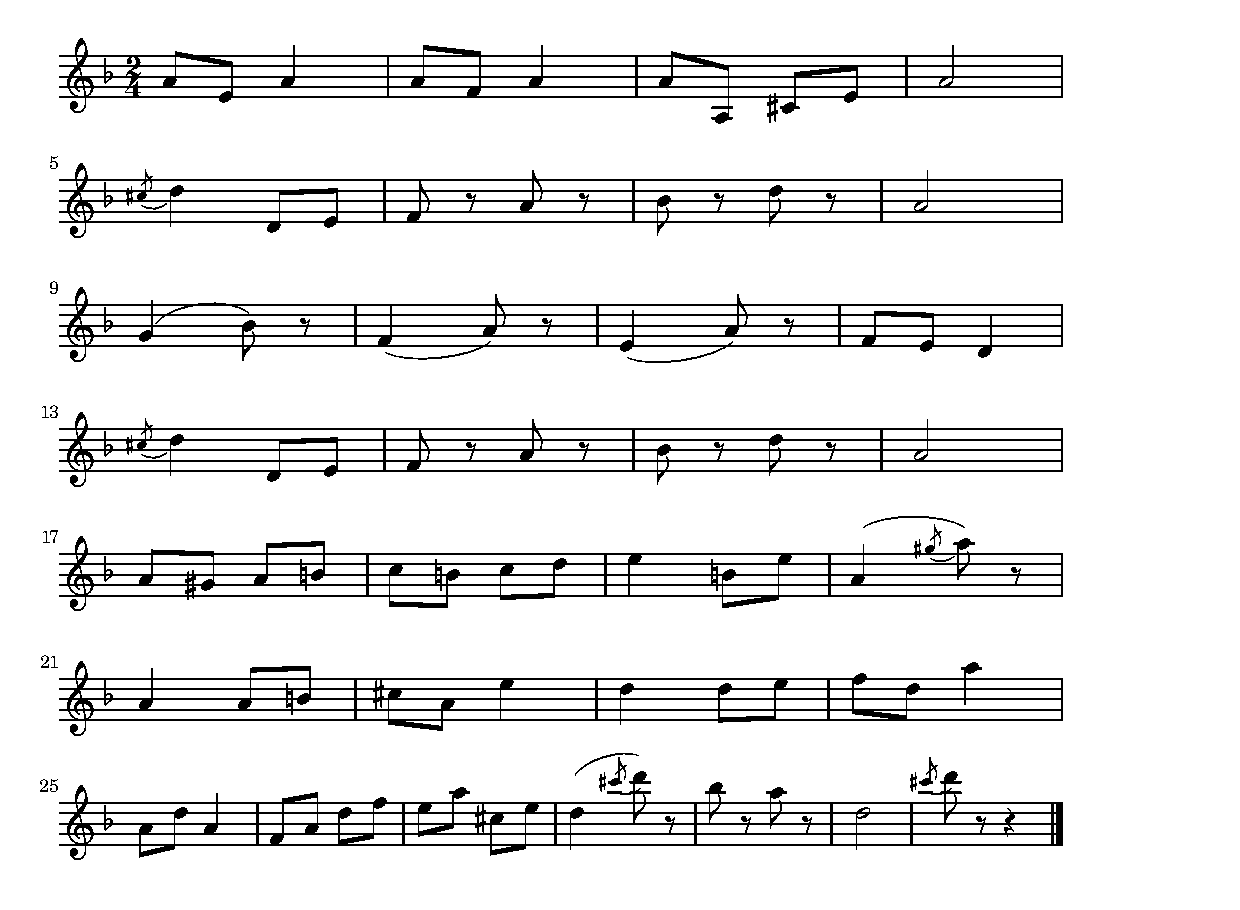
\includegraphics[clip]{csikospost_crop.pdf}

\vspace{-10mm} \hspace{10mm}
クシコス・ポスト(ネッケ)
\index{くしこす@クシコス・ポスト(ネッケ)}

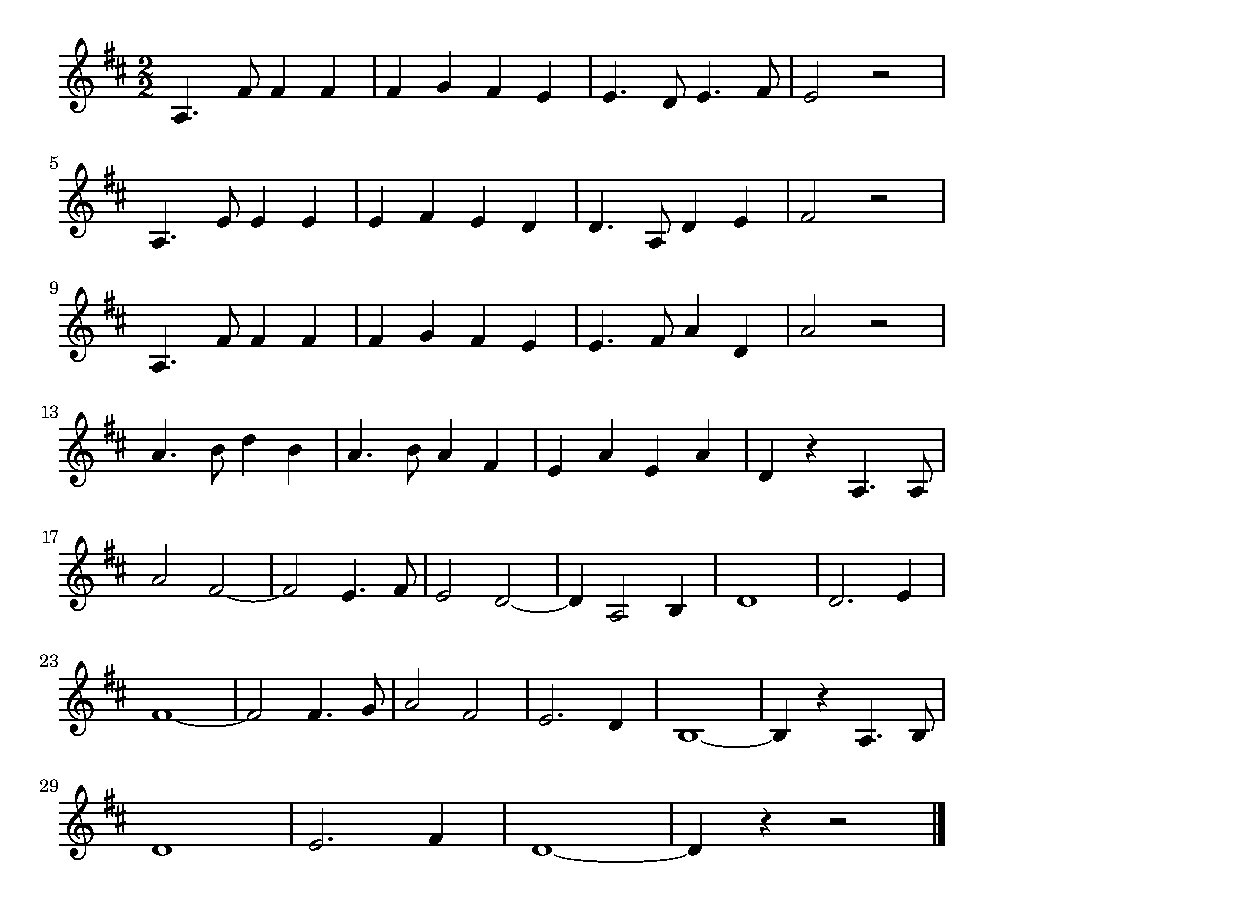
\includegraphics[clip]{gunkan_crop.pdf}

\vspace{-10mm} \hspace{10mm}
軍艦マーチ(まもるもせむるも)
\index{ぐんかん@軍艦マーチ(まもるもせむるも)}

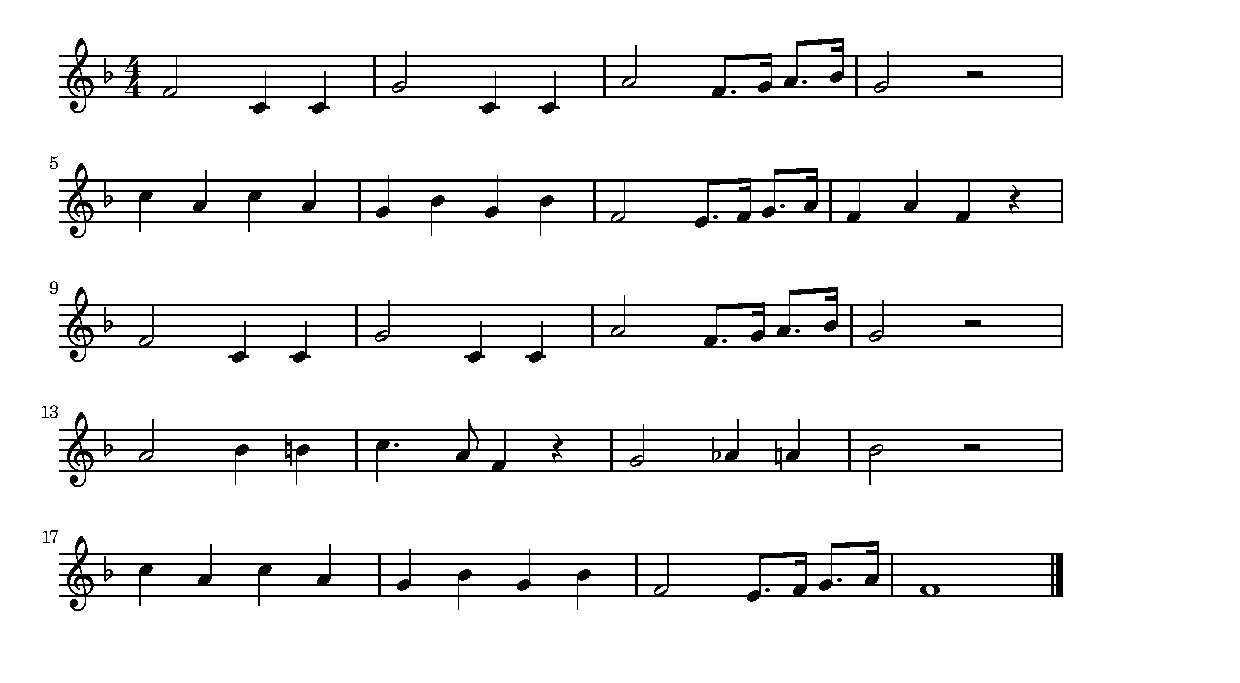
\includegraphics[clip]{koitowadonna_crop.pdf}

\vspace{-10mm} \hspace{10mm}
恋とはどんなものかしら(モーツアルト。フィガロの結婚より)
\index{こいとは@恋とはどんなものかしら(モーツアルト。フィガロの結婚より)}
\index{もーつぁると@恋とはどんなものかしら(モーツアルト。フィガロの結婚より)}

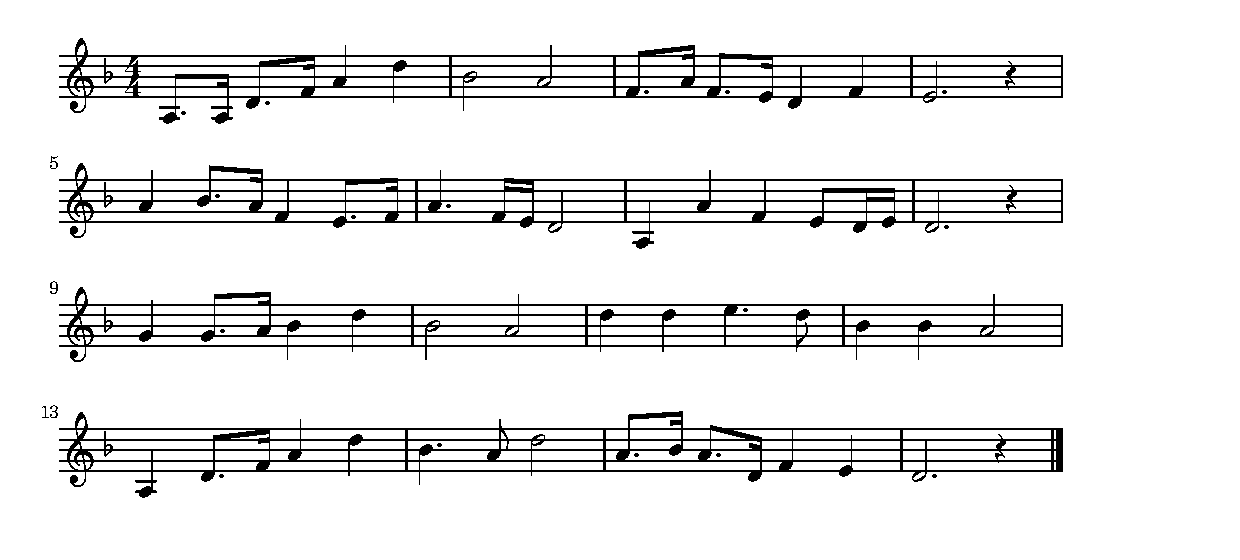
\includegraphics[clip]{doukinosakura_crop.pdf}

\vspace{-10mm} \hspace{10mm}
同期の桜(きさまとおれとは)
\index{どうき@同期の桜(きさまとおれとは)}

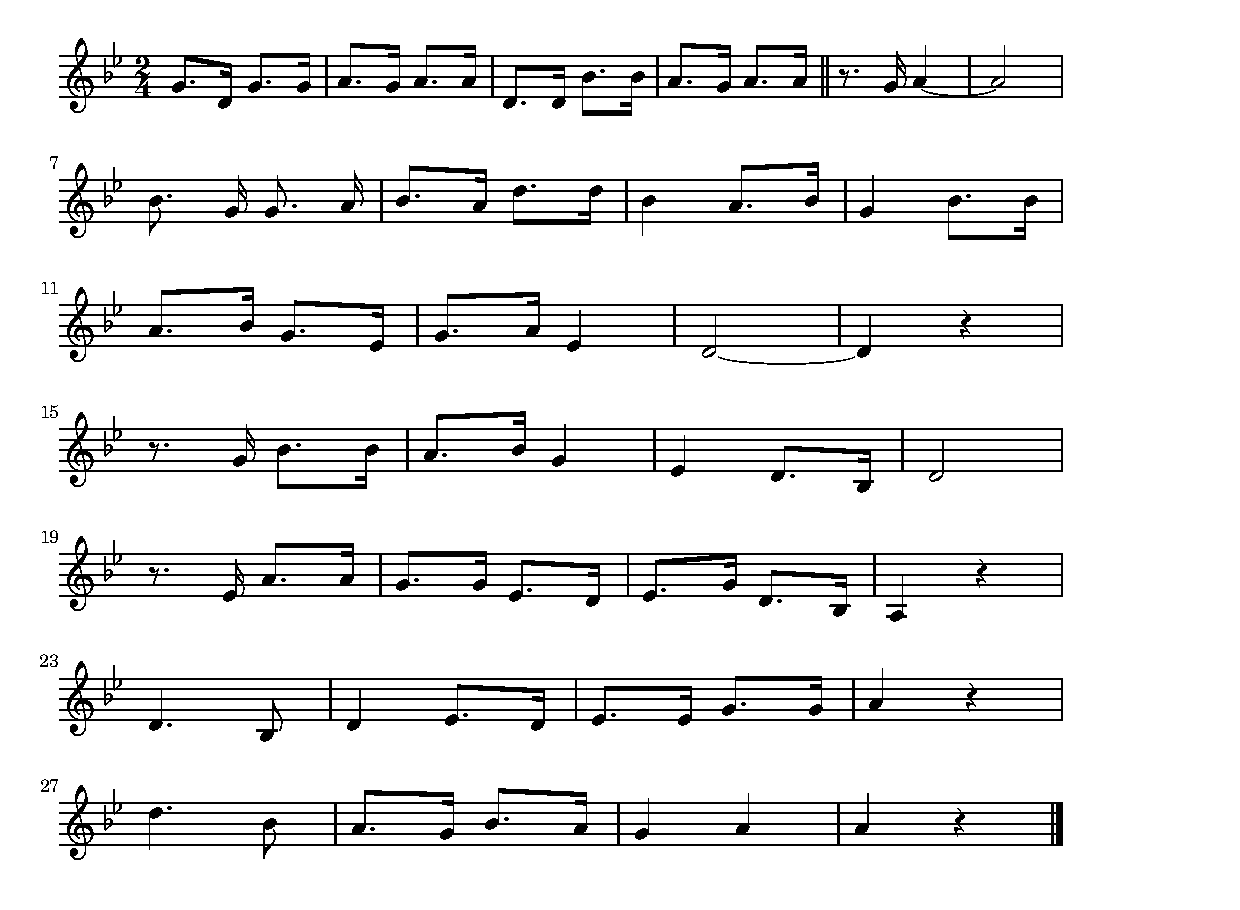
\includegraphics[clip]{tokyoondo_crop.pdf}

\vspace{-10mm} \hspace{10mm}
東京音頭(とうきょうおんど。はあーおどりおどるならちょいと)
\index{とうきょう@東京音頭(とうきょうおんど。はあーおどりおどるならちょいと)}

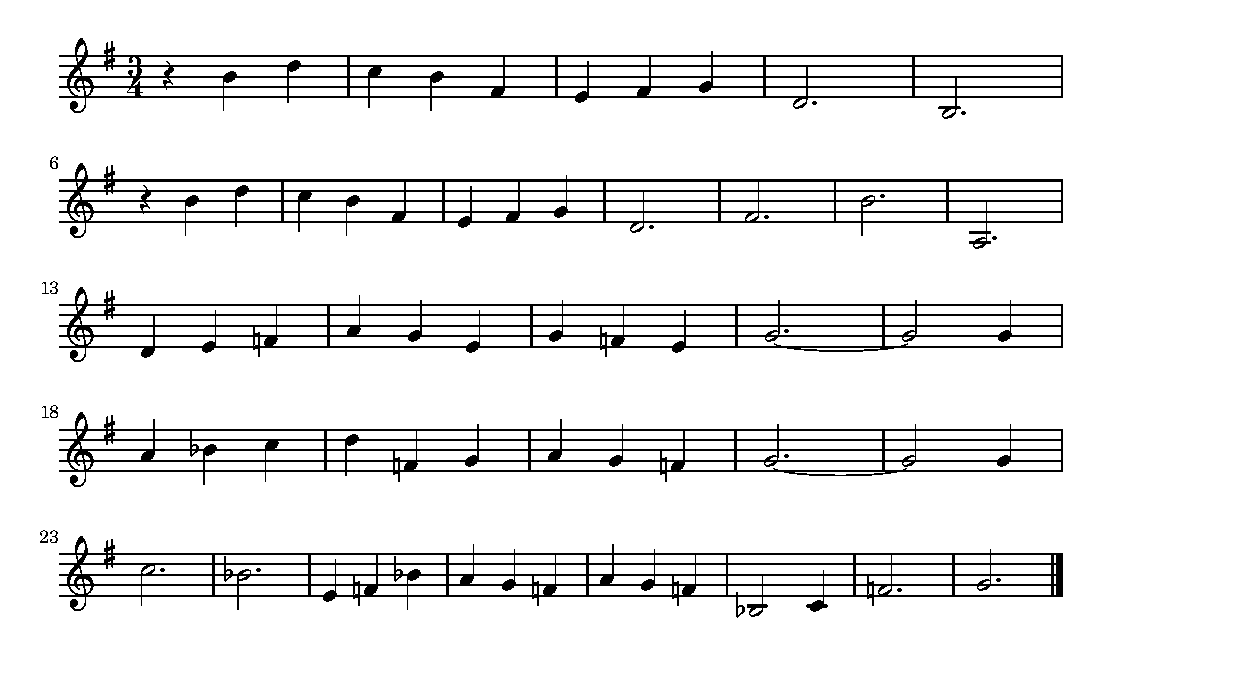
\includegraphics[clip]{gymnopedies_crop.pdf}

\vspace{-10mm} \hspace{10mm}
ジムノペディ1番(サティ)
\index{じむ@ジムノペディ1番(サティ)}
\index{さてぃ@ジムノペディ1番(サティ)}

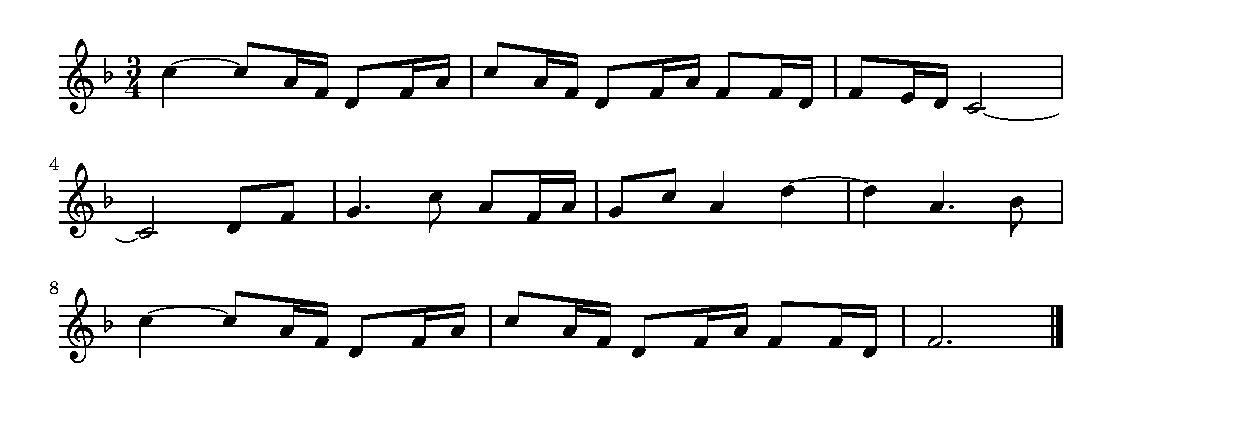
\includegraphics[clip]{amairodebussy_crop.pdf}

\vspace{-10mm} \hspace{10mm}
亜麻色の髪の乙女(ドビュッシー)
\index{あまいろ@亜麻色の髪の乙女(ドビュッシー)}
\index{どびゅっしー@亜麻色の髪の乙女(ドビュッシー)}

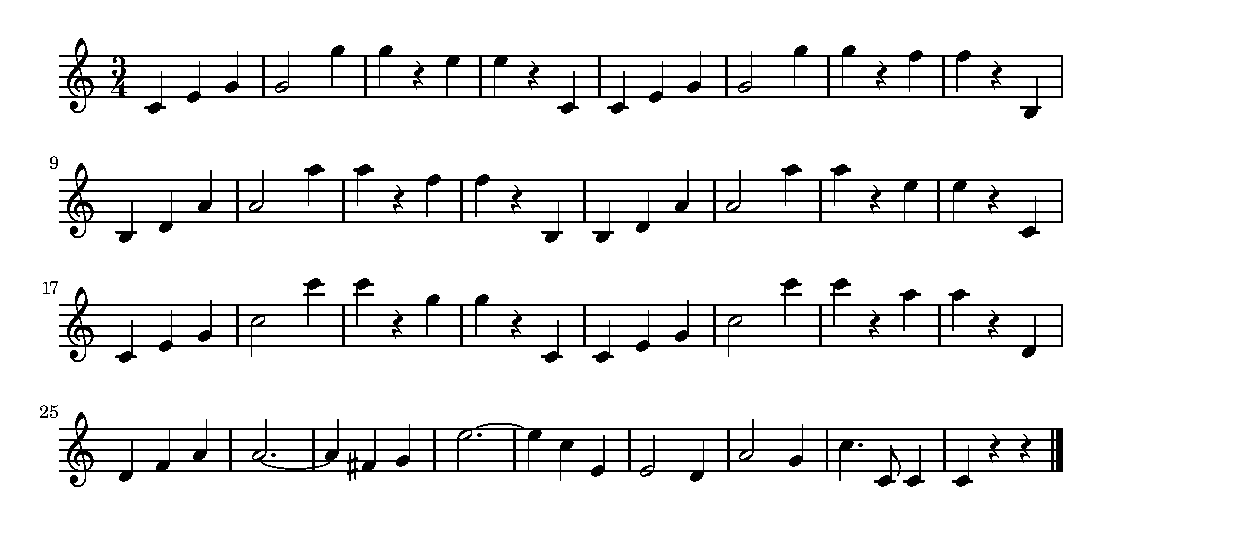
\includegraphics[clip]{donau_crop.pdf}

\vspace{-10mm} \hspace{10mm}
美しき青きドナウ(ヨハン・シュトラウス2世)
\index{うつくしき@美しき青きドナウ(ヨハン・シュトラウス2世)}

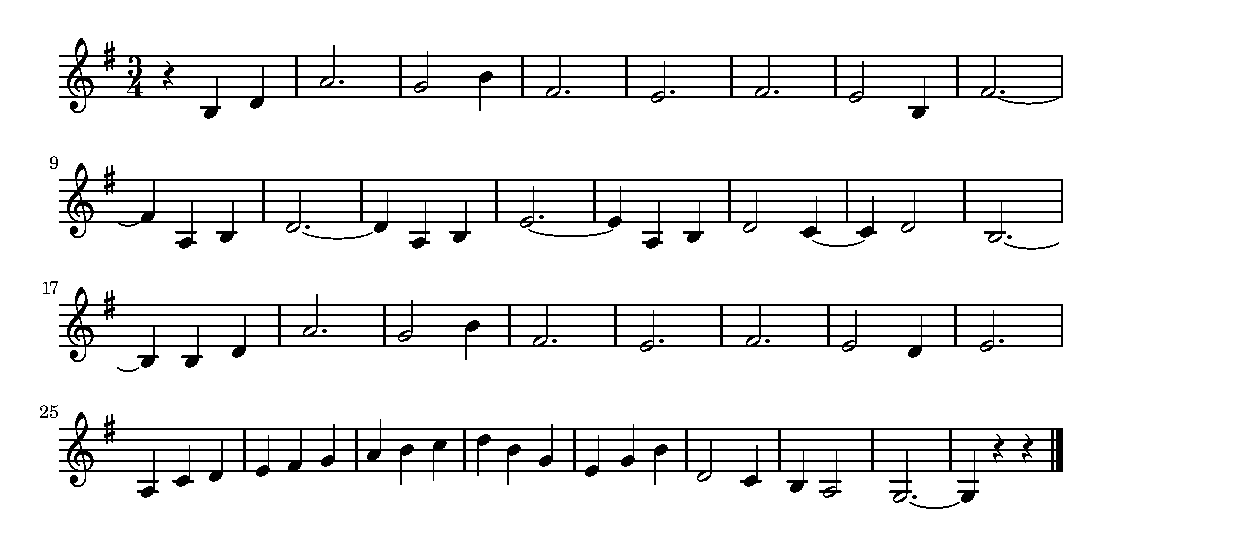
\includegraphics[clip]{jeteveux_crop.pdf}

\vspace{-10mm} \hspace{10mm}
ジュ・トゥ・ヴ(エリック・サティ)
\index{じゅとぶ@ジュ・トゥ・ヴ(エリック・サティ)}
\index{さてぃ@ジュ・トゥ・ヴ(エリック・サティ)}

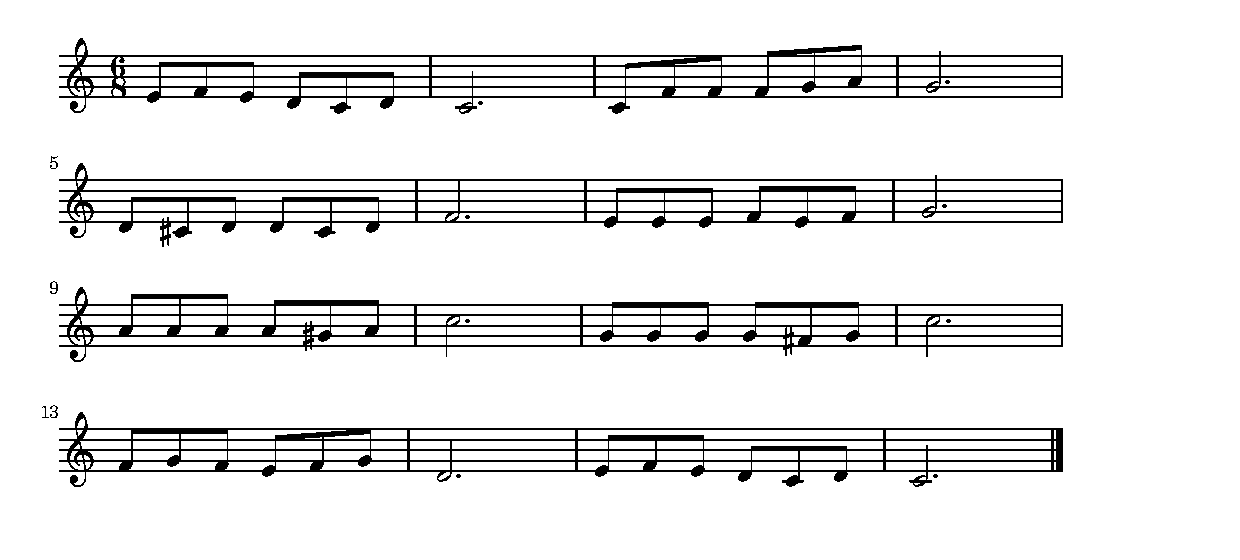
\includegraphics[clip]{mozartkomori_crop.pdf}

\vspace{-10mm} \hspace{10mm}
モーツァルトの子守歌
\index{もーつ@モーツァルトの子守歌}
\index{こもりうた@モーツァルトの子守歌}

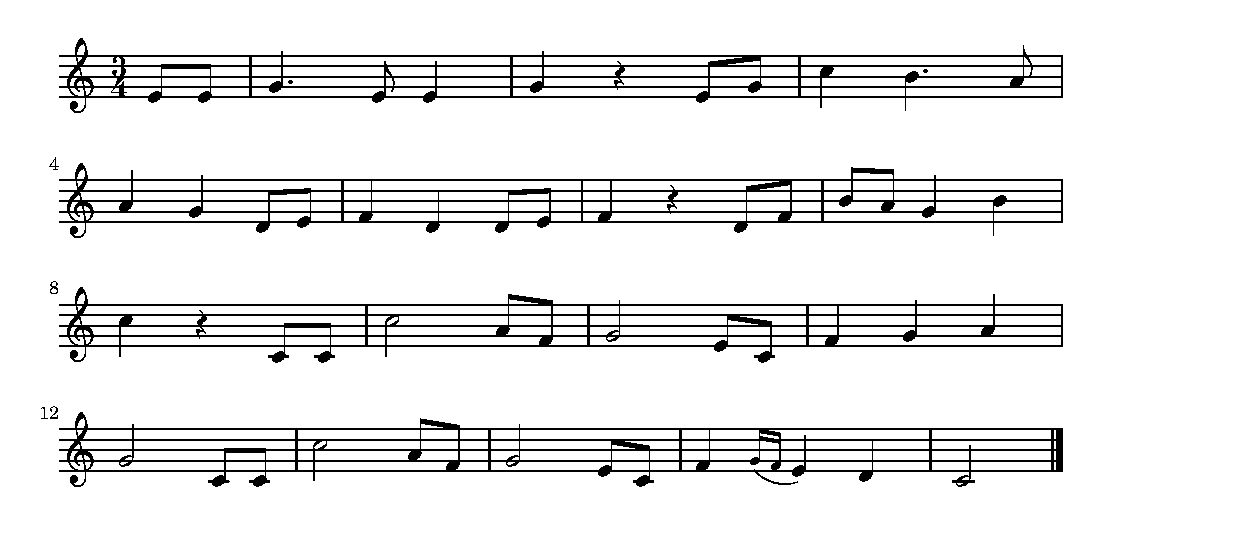
\includegraphics[clip]{brahmskomori_crop.pdf}

\vspace{-10mm} \hspace{10mm}
ブラームスの子守歌
\index{ぶらーむす@ブラームスの子守歌}
\index{こもりうた@ブラームスの子守歌}

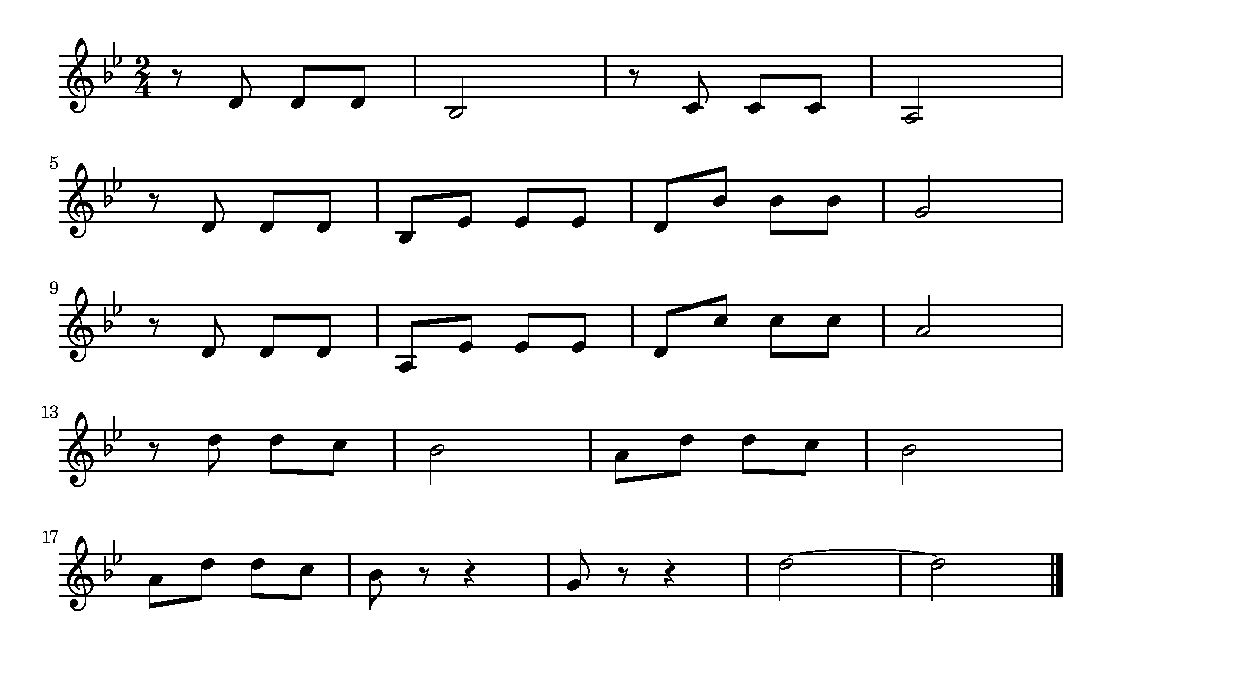
\includegraphics[clip]{unmei_crop.pdf}

\vspace{-10mm} \hspace{10mm}
運命(ベートーベン交響曲5番)
\index{うんめい@運命(ベートーベン交響曲5番)}

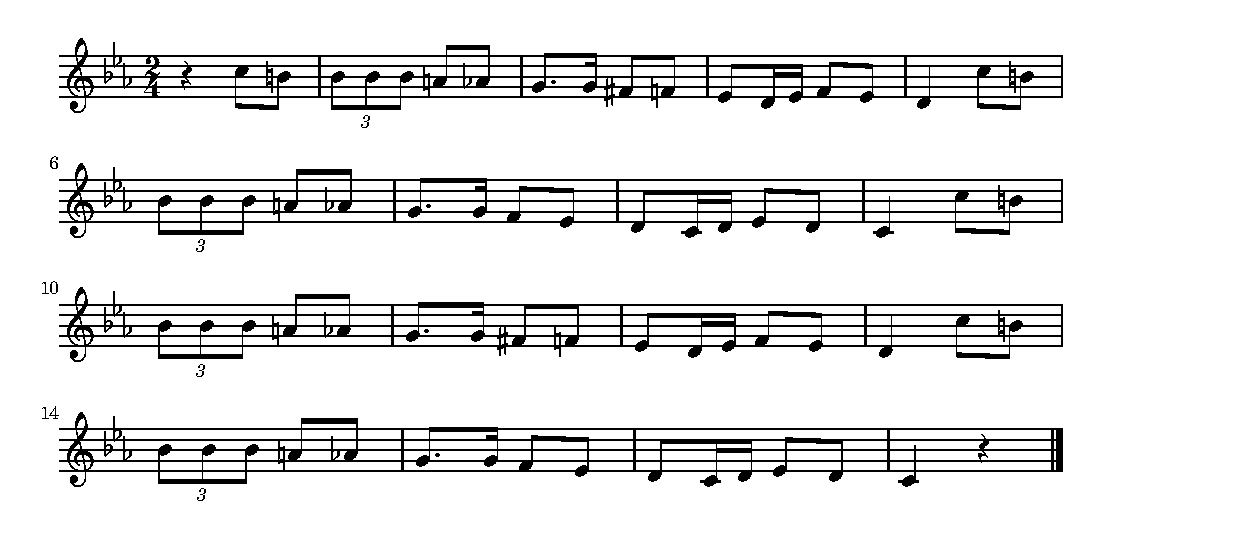
\includegraphics[clip]{habanera_crop.pdf}

\vspace{-10mm} \hspace{10mm}
ハバネラ(ビゼー。カルメンより)
\index{はばねら@ハバネラ(ビゼー。カルメンより)}

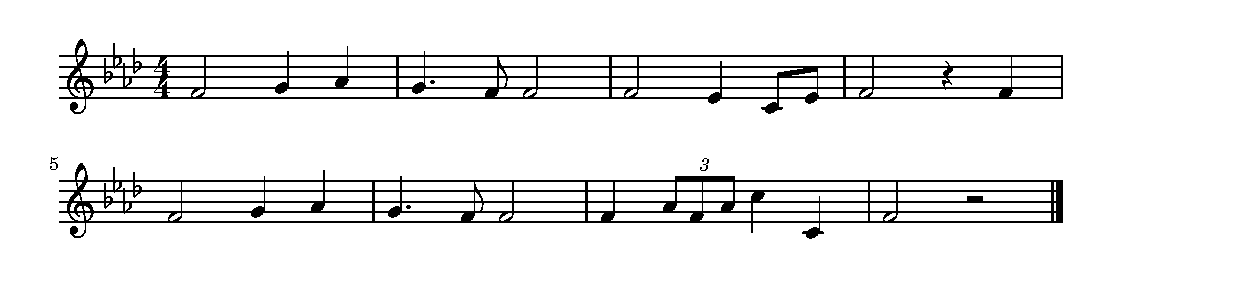
\includegraphics[clip]{shinsekai_crop.pdf}

\vspace{-10mm} \hspace{10mm}
新世界(ドヴォルザーク)
\index{しんせかい@新世界(ドヴォルザーク)}

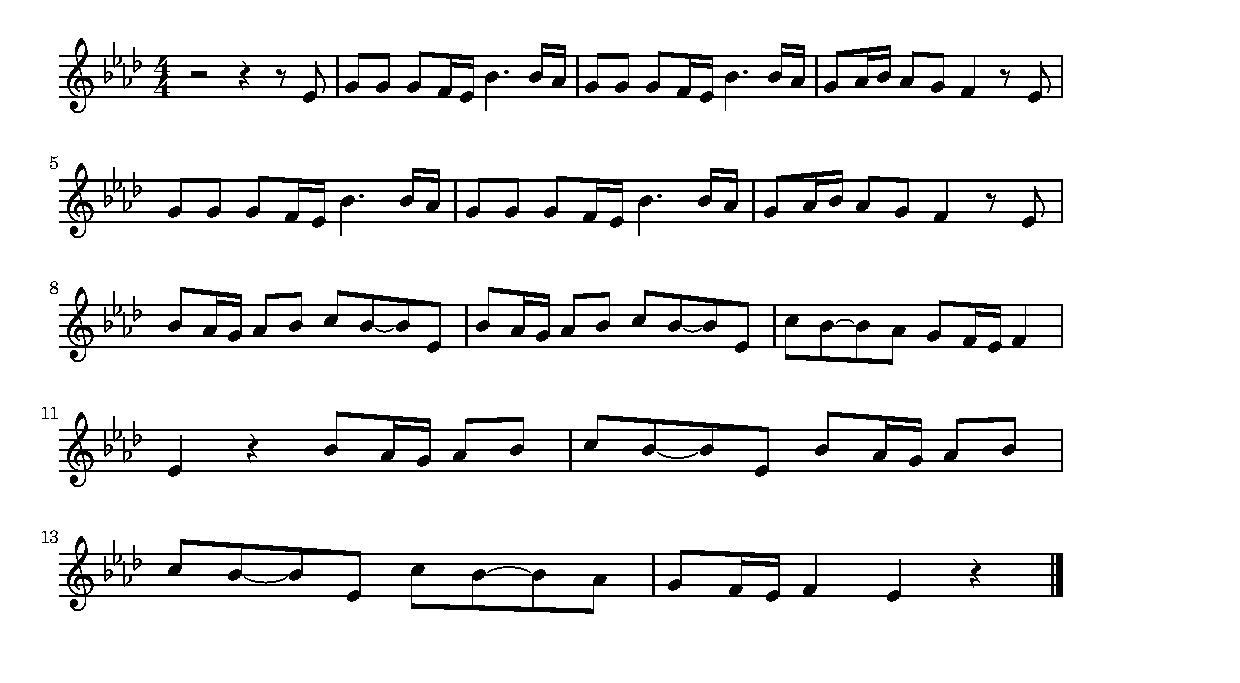
\includegraphics[clip]{vivaldishiki_crop.pdf}

\vspace{-10mm} \hspace{10mm}
ヴィヴァルディ四季より春
\index{ゔぃゔぁるでぃ@ヴィヴァルディ四季より春}

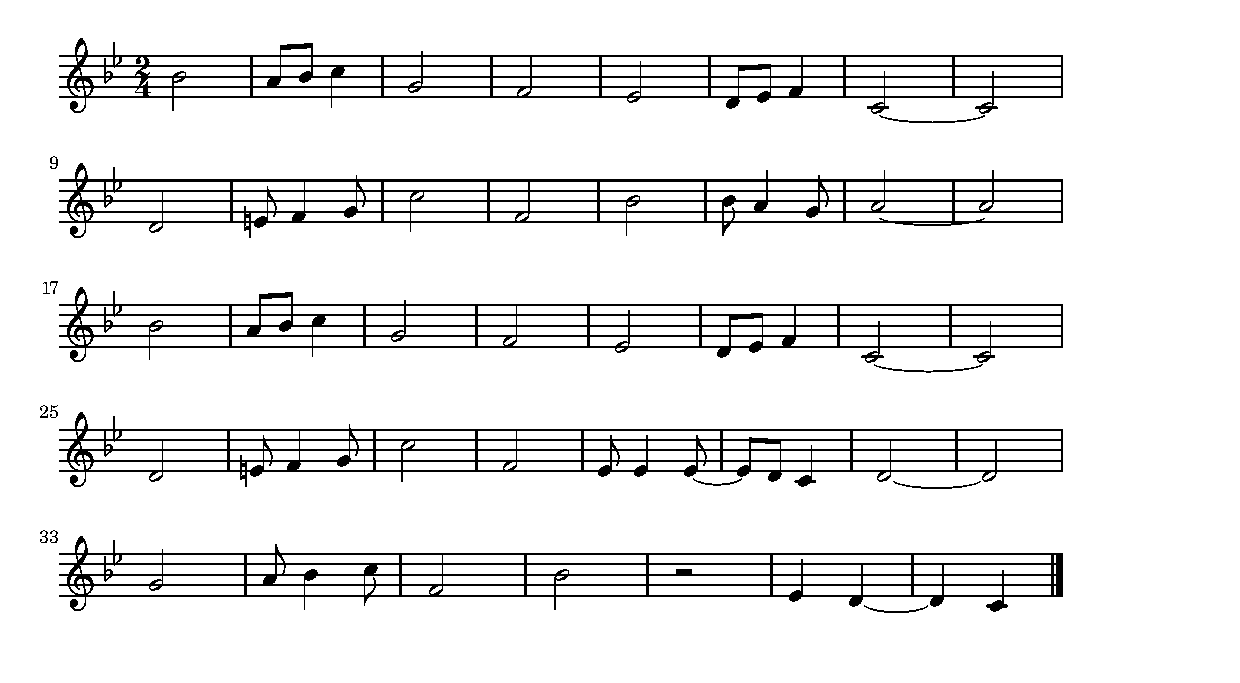
\includegraphics[clip]{ifudodo_crop.pdf}

\vspace{-10mm} \hspace{10mm}
威風堂々(エルガー)
\index{いふうどうどう@威風堂々(エルガー)}

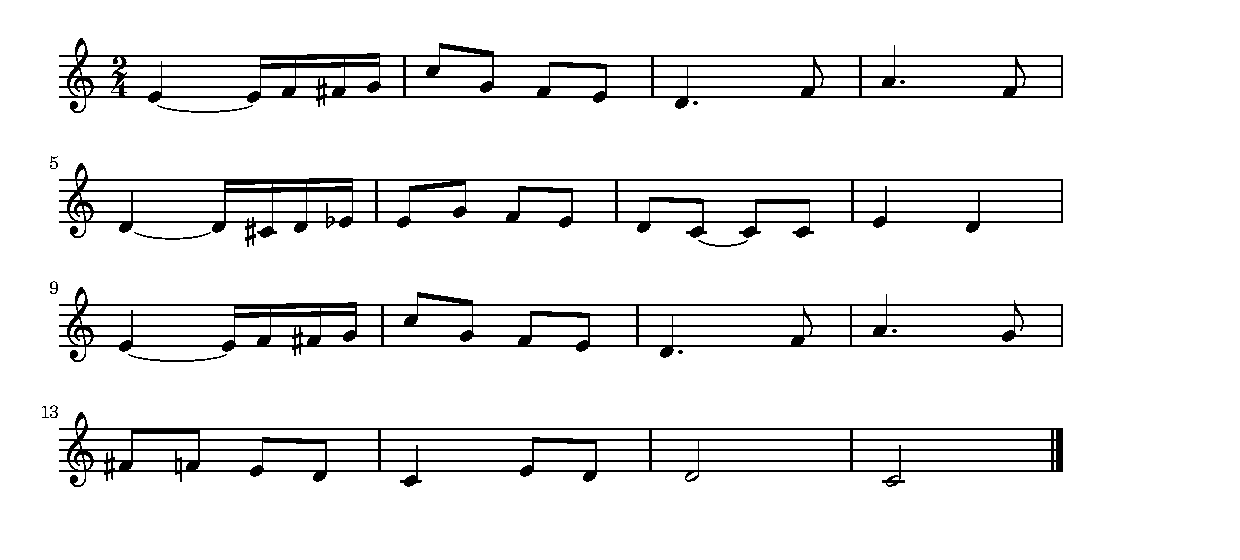
\includegraphics[clip]{mendelsharunouta_crop.pdf}

\vspace{-10mm} \hspace{10mm}
春の歌(メンデルスゾーン)
\index{はるのうた@春の歌(メンデルスゾーン)}

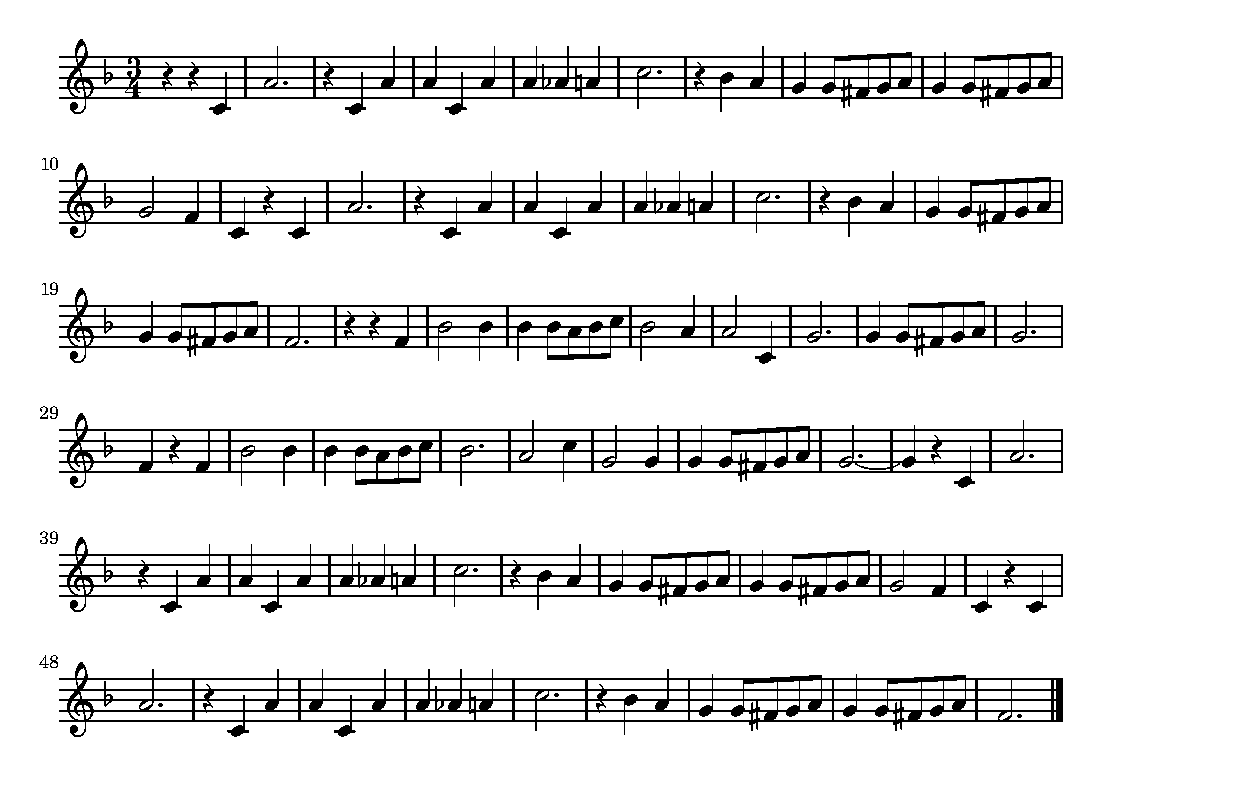
\includegraphics[clip]{kanpai_crop.pdf}

\vspace{-10mm} \hspace{10mm}
乾杯の歌(ヴェルディ)
\index{かんぱい@乾杯の歌(ヴェルディ)}

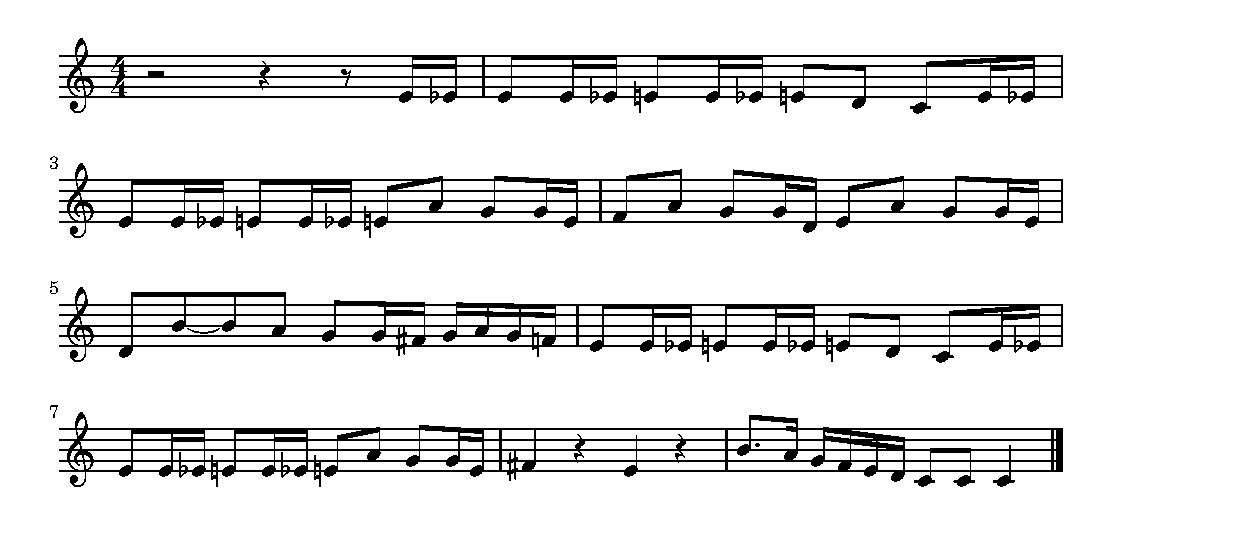
\includegraphics[clip]{radetzky_crop.pdf}

\vspace{-10mm} \hspace{10mm}
ラデツキー行進曲(ヨハン・シュトラウス1世)
\index{らでつきー@ラデツキー行進曲(ヨハン・シュトラウス1世)}

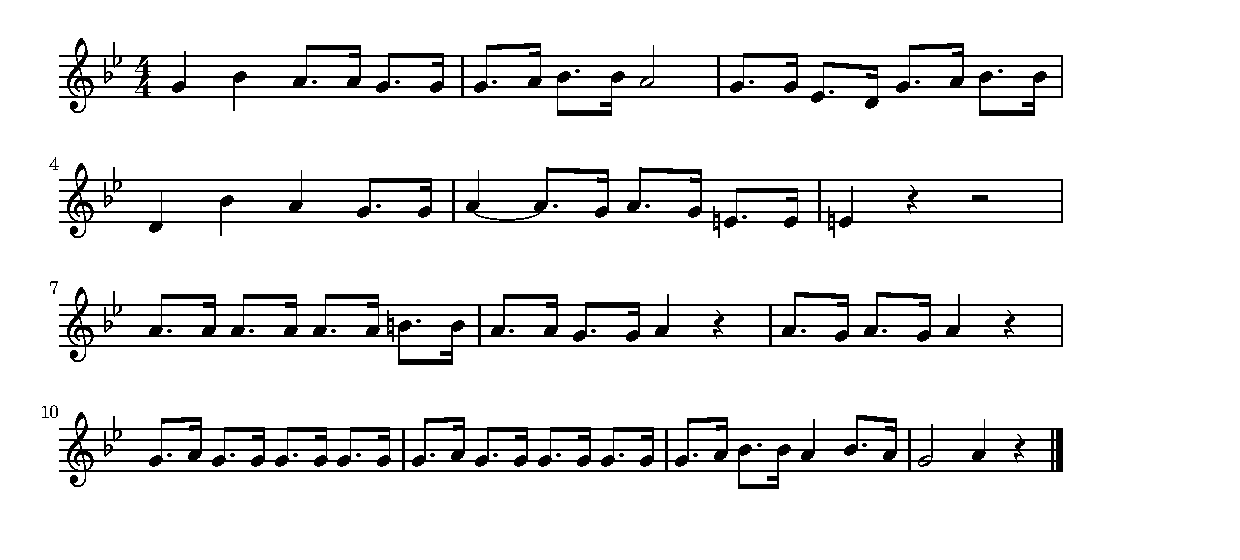
\includegraphics[clip]{zuizui_crop.pdf}

\vspace{-10mm} \hspace{10mm}
ずいずいずっころばし
\index{ずいずい@ずいずいずっころばし}

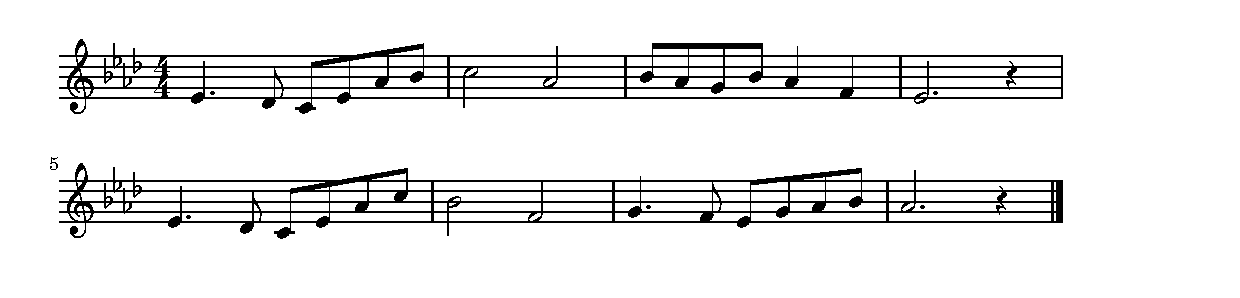
\includegraphics[clip]{moeroyo_crop.pdf}

\vspace{-10mm} \hspace{10mm}
燃えろよ燃えろよ
\index{もえろよ@燃えろよ燃えろよ}

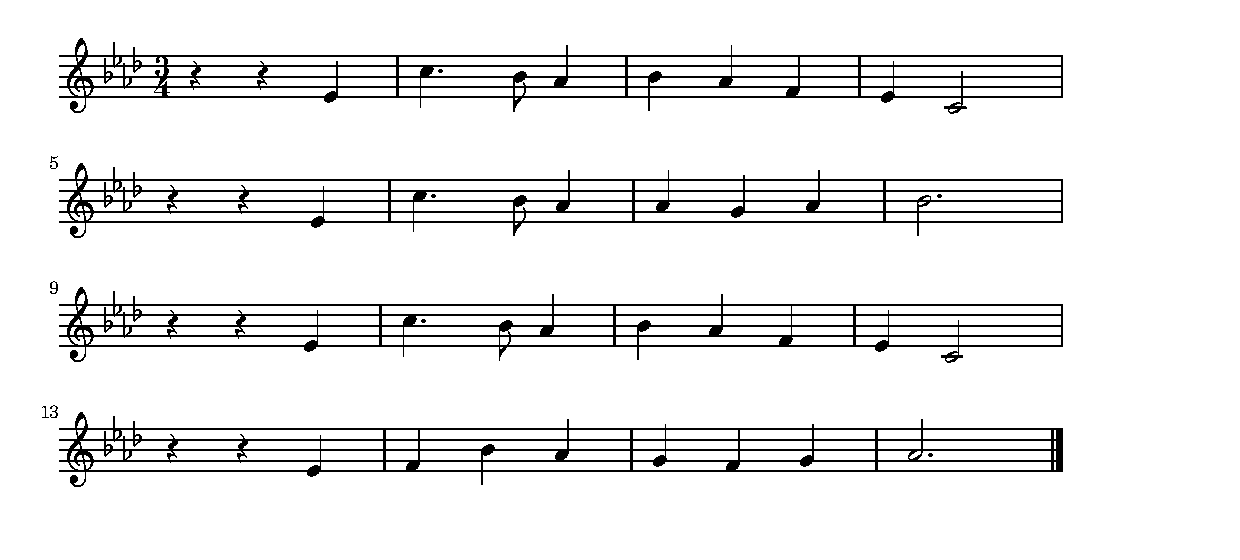
\includegraphics[clip]{mybonnie_crop.pdf}

\vspace{-10mm} \hspace{10mm}
マイボニー(My Bonnie Lies Over the Ocean)
\index{まいぼにー@マイボニー(My Bonnie Lies Over the Ocean)}

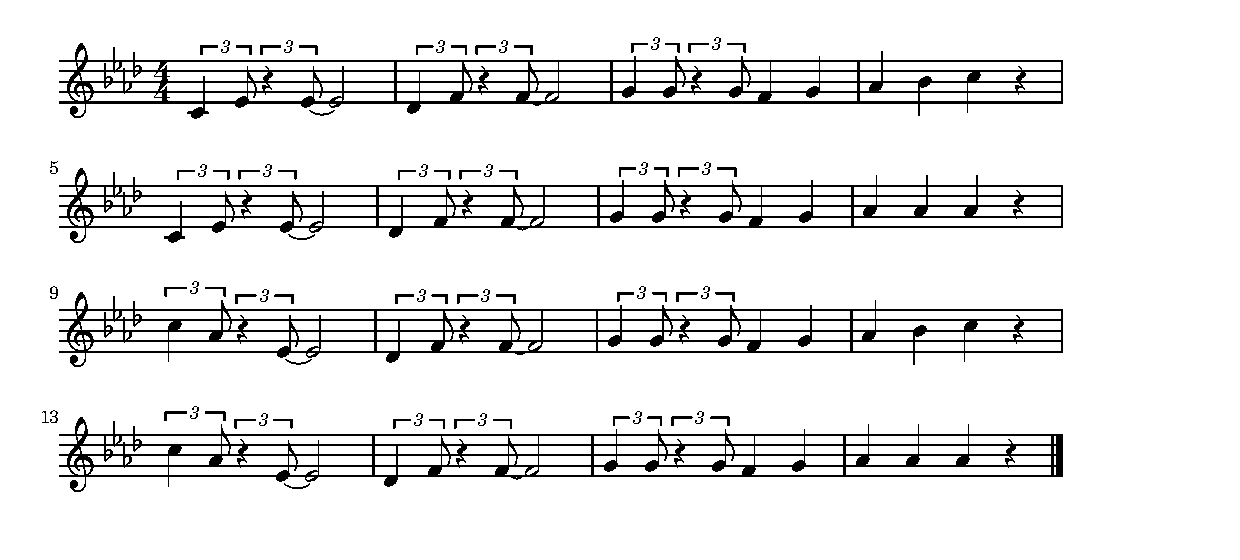
\includegraphics[clip]{chairo_crop.pdf}

\vspace{-10mm} \hspace{10mm}
茶色の小瓶
\index{ちゃいろの@茶色の小瓶}

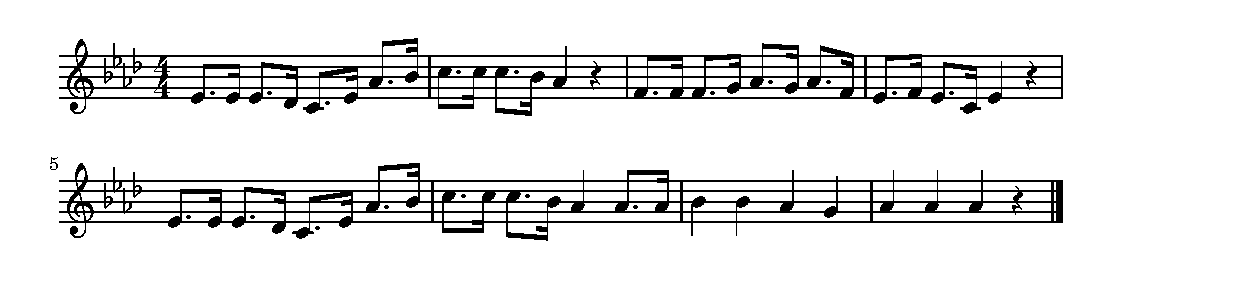
\includegraphics[clip]{gonbe_crop.pdf}

\vspace{-10mm} \hspace{10mm}
権兵衛さんの赤ちゃん(ごんべえさんのあかちゃんが)
\index{ごんべえ@権兵衛さんの赤ちゃん(ごんべえさんのあかちゃんが)}

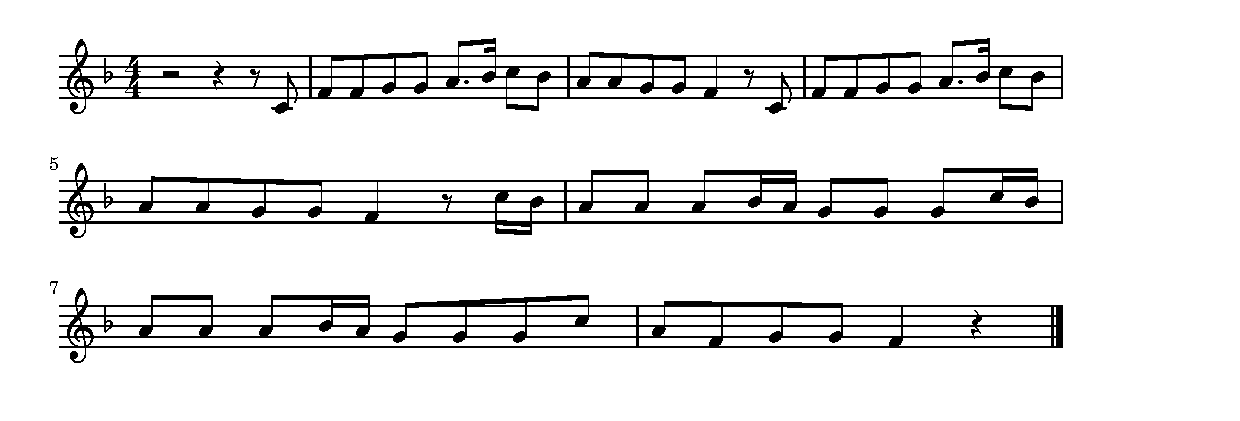
\includegraphics[clip]{yamanoongakuka_crop.pdf}

\vspace{-10mm} \hspace{10mm}
山の音楽家(わたしゃおんがくかやまのこりす)
\index{やまのおんがくか@山の音楽家(わたしゃおんがくかやまのこりす)}

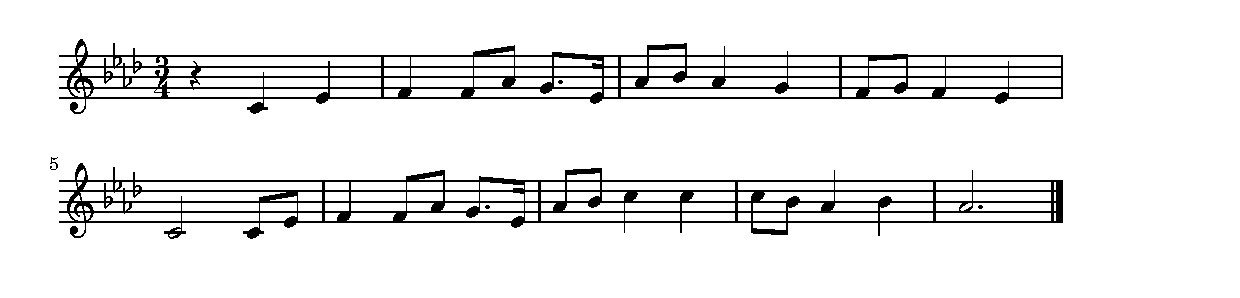
\includegraphics[clip]{mokusei_crop.pdf}

\vspace{-10mm} \hspace{10mm}
木星(ホルスト「惑星」よりジュピター)
\index{もくせい@木星(ホルスト「惑星」よりジュピター)}

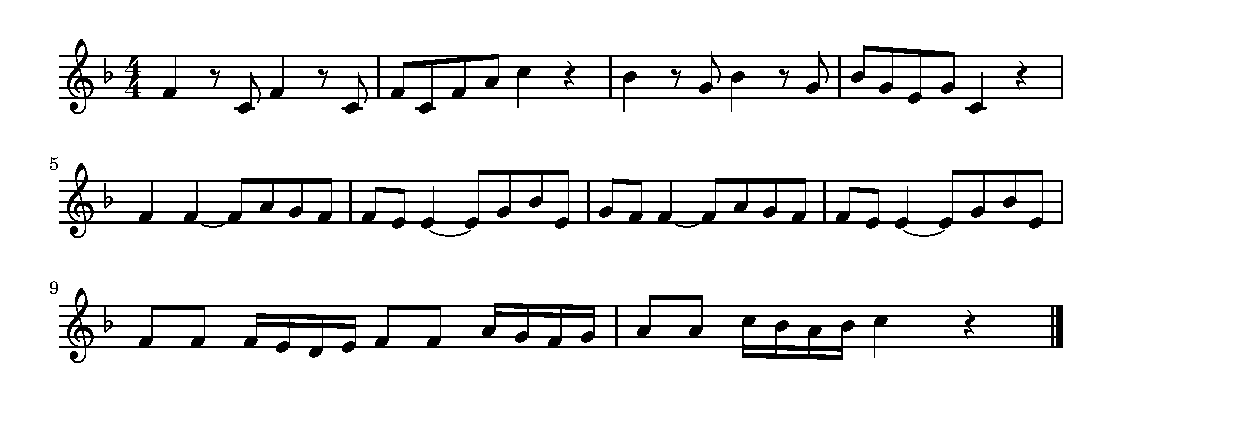
\includegraphics[clip]{eineclinenacht_crop.pdf}

\vspace{-10mm} \hspace{10mm}
アイネ・クライネ・ナハト・ムジーク(モーツァルト)
\index{あいねくらいね@アイネ・クライネ・ナハト・ムジーク(モーツァルト)}

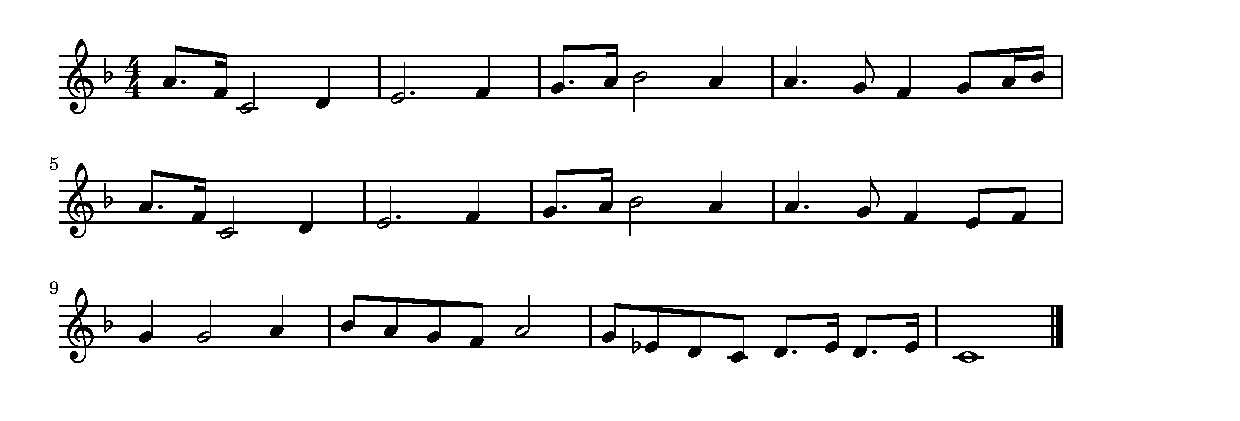
\includegraphics[clip]{amadare_crop.pdf}

\vspace{-10mm} \hspace{10mm}
雨だれの前奏曲(ショパン)
\index{あまだれ@雨だれの前奏曲(ショパン)}

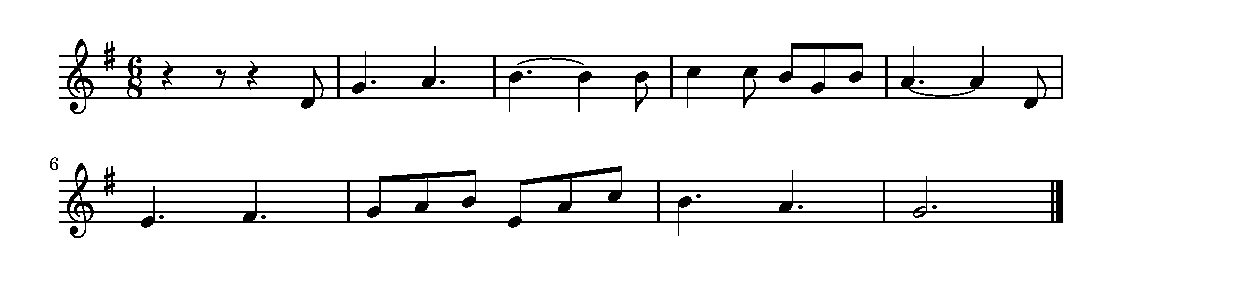
\includegraphics[clip]{ainoyorokobi_crop.pdf}

\vspace{-10mm} \hspace{10mm}
愛の喜び(マルティーニ)
\index{あいのよろこび@愛の喜び(マルティーニ)}

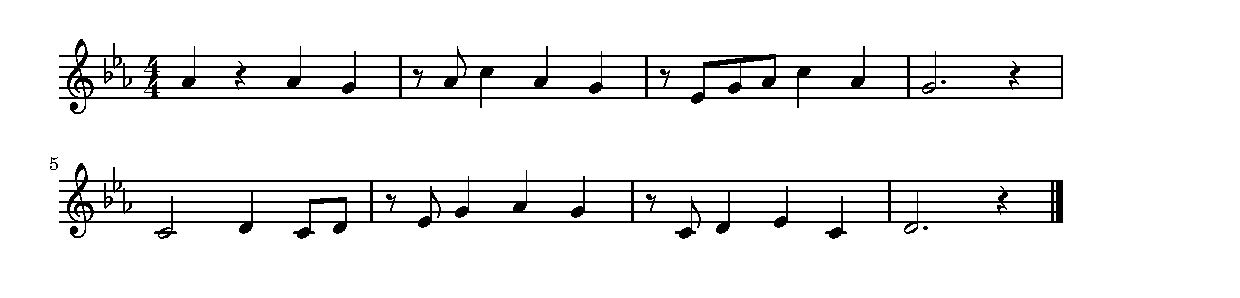
\includegraphics[clip]{edokomori_crop.pdf}

\vspace{-10mm} \hspace{10mm}
江戸の子守唄(ねんねんころりよおころりよ)
\index{えど@江戸の子守唄(ねんねんころりよおころりよ)}
\index{こもりうた@江戸の子守唄(ねんねんころりよおころりよ)}

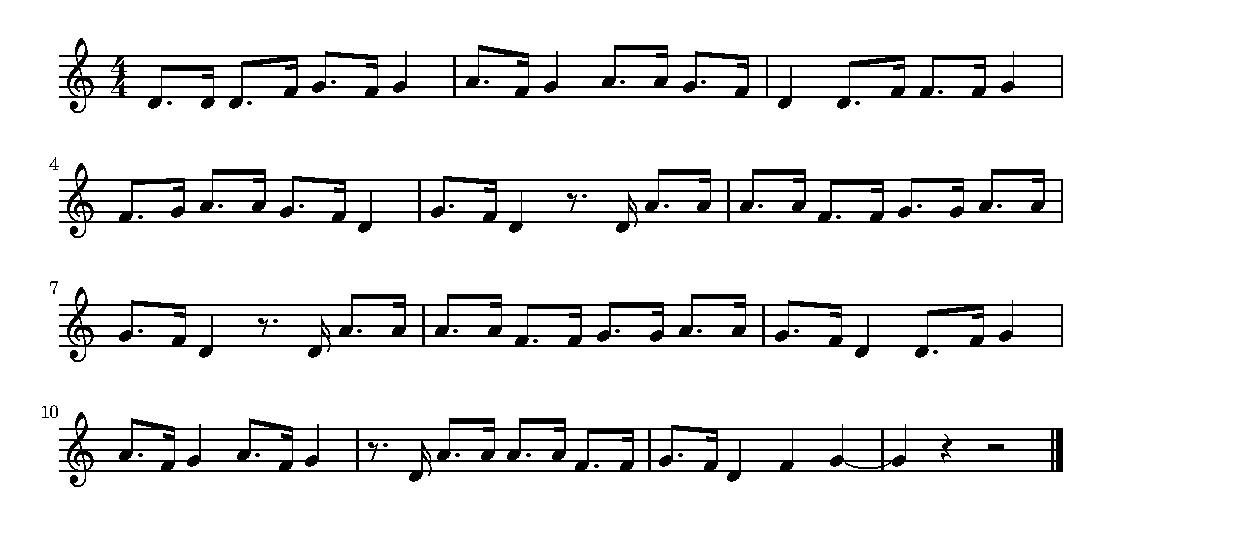
\includegraphics[clip]{antagata_crop.pdf}

\vspace{-10mm} \hspace{10mm}
あんたがたどこさ(ひごさひごどこさくまもとさ)
\index{あんたがた@あんたがたどこさ(ひごさひごどこさくまもとさ)}

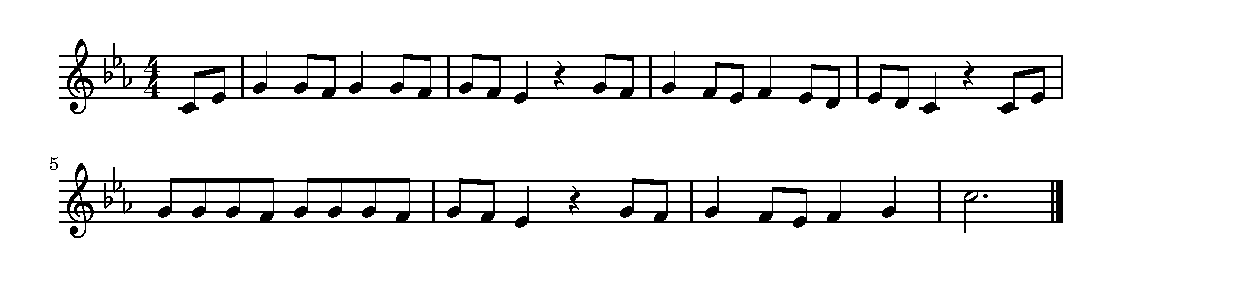
\includegraphics[clip]{isshukan_crop.pdf}

\vspace{-10mm} \hspace{10mm}
一週間(にちようびにいちばにでかけ)
\index{いっしゅうかん@一週間(にちようびにいちばにでかけ)}

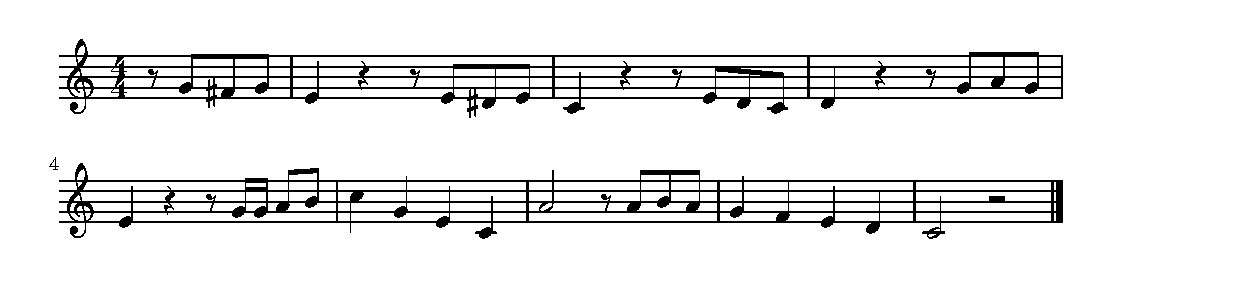
\includegraphics[clip]{morinokuma_crop.pdf}

\vspace{-10mm} \hspace{10mm}
森のくまさん(あるひもりのなかくまさんにであった)
\index{もり@森のくまさん(あるひもりのなかくまさんにであった)}

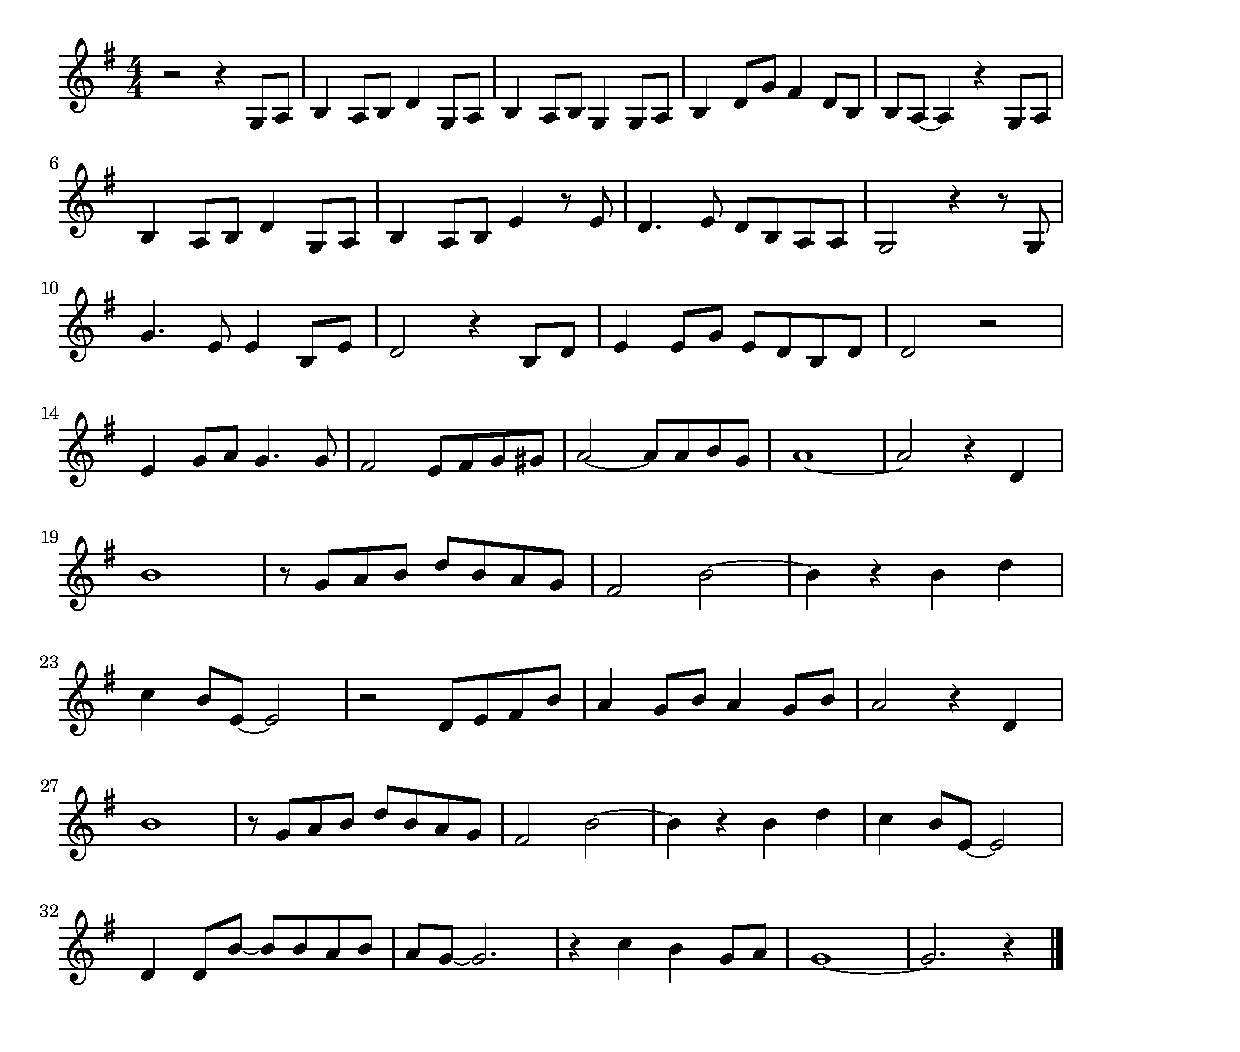
\includegraphics[clip]{kawanonagare_crop.pdf}

\vspace{-10mm} \hspace{10mm}
川の流れのように(しらずしらずあるいてきた)
\index{かわ@川の流れのように(しらずしらずあるいてきた)}

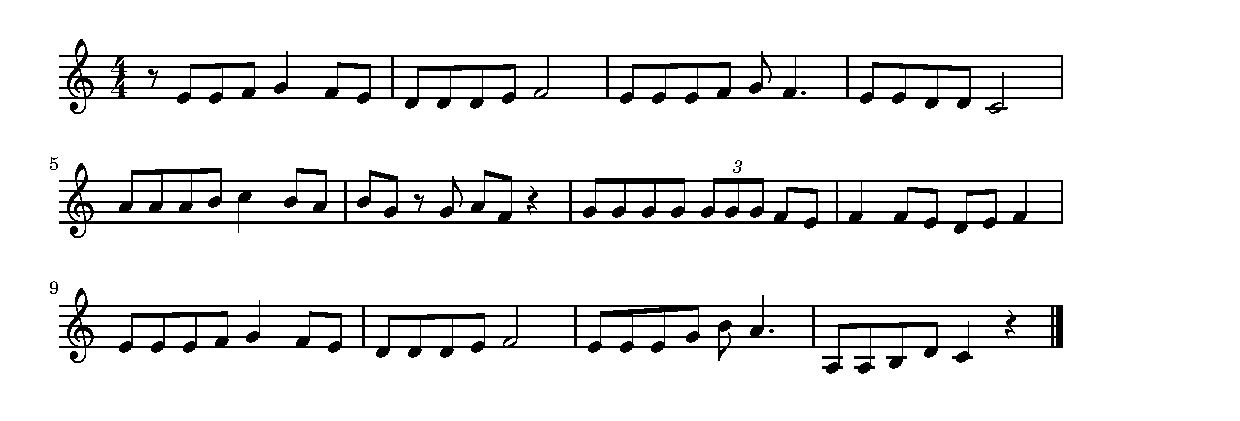
\includegraphics[clip]{natsunoomoide_crop.pdf}

\vspace{-10mm} \hspace{10mm}
夏の思い出(なつがくればおもいだす)
\index{なつ@夏の思い出(なつがくればおもいだす)}

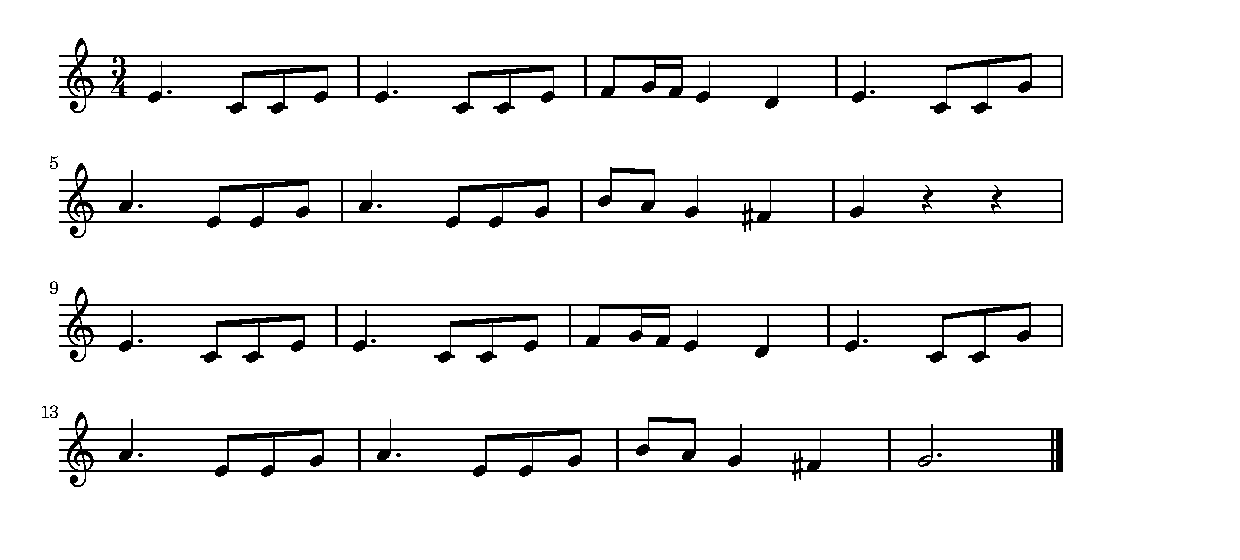
\includegraphics[clip]{waltzbrahms_crop.pdf}

\vspace{-10mm} \hspace{10mm}
ブラームスのワルツ(円舞曲)
\index{ぶら@ブラームスのワルツ(円舞曲)}

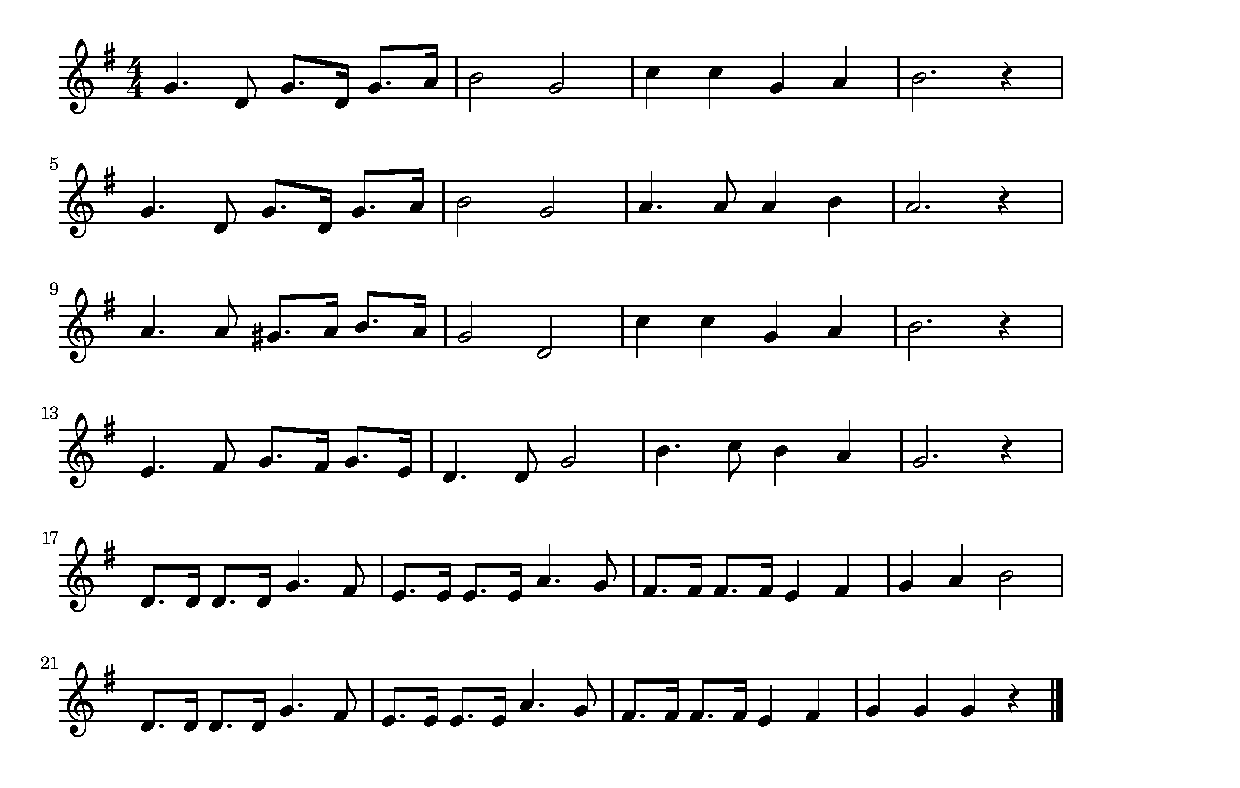
\includegraphics[clip]{senrowa_crop.pdf}

\vspace{-10mm} \hspace{10mm}
線路は続くよどこまでも(せんろはつづくよどこまでも)
\index{せんろ@線路は続くよどこまでも(せんろはつづくよどこまでも)}

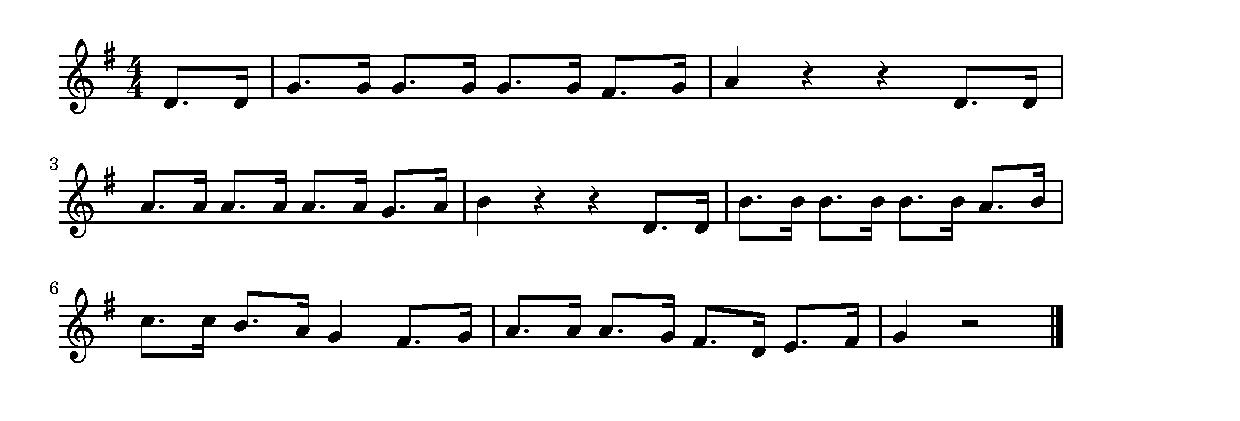
\includegraphics[clip]{shiawasenara_crop.pdf}

\vspace{-10mm} \hspace{10mm}
幸せなら手をたたこう(しあわせならてをたたこう)
\index{しあわせ@幸せなら手をたたこう(しあわせならてをたたこう)}


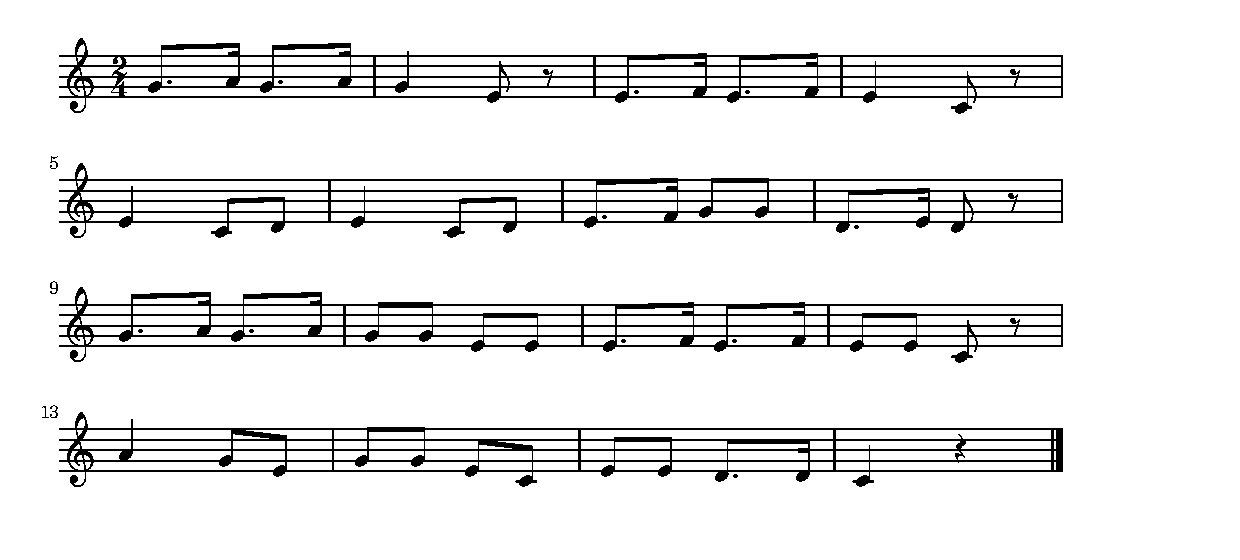
\includegraphics[clip]{yukiyakonko_crop.pdf}

\vspace{-10mm} \hspace{10mm}
雪(ゆきやこんこあられやこんこ)
\index{ゆき@雪(ゆきやこんこあられやこんこ)}

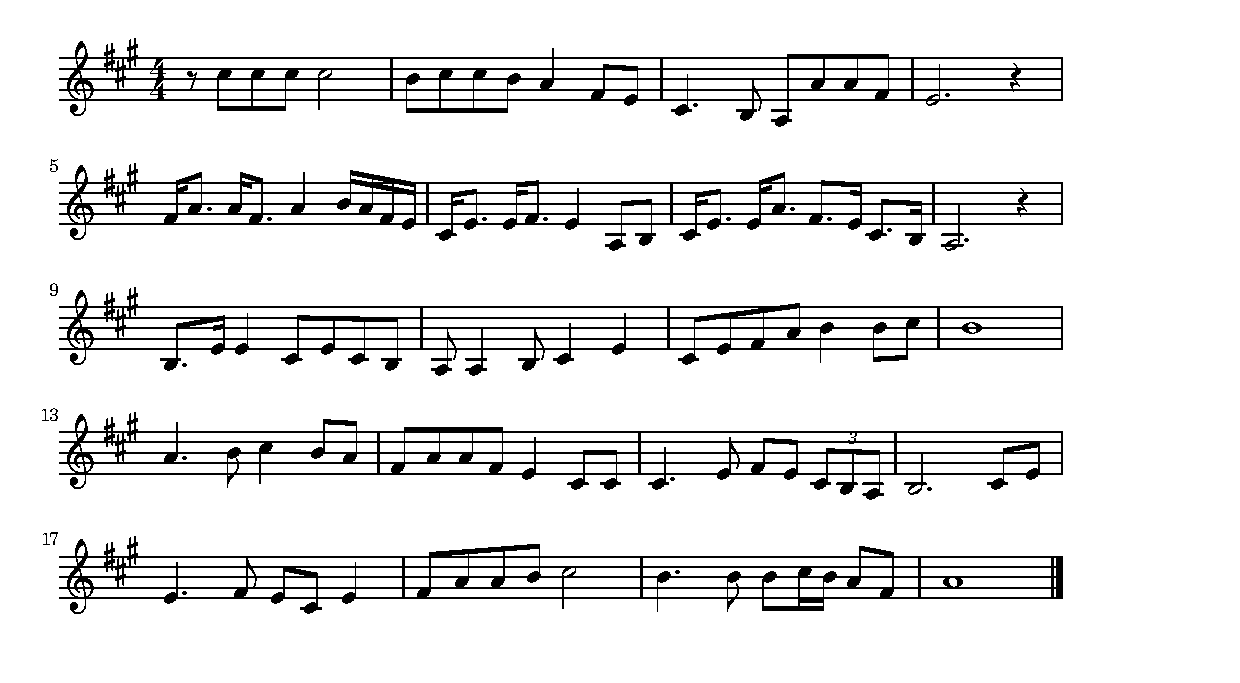
\includegraphics[clip]{kitaguninoharu_crop.pdf}

\vspace{-10mm} \hspace{10mm}
北国の春(しらかばあおぞらみなみかぜ)
\index{きたぐに@北国の春(しらかばあおぞらみなみかぜ)}

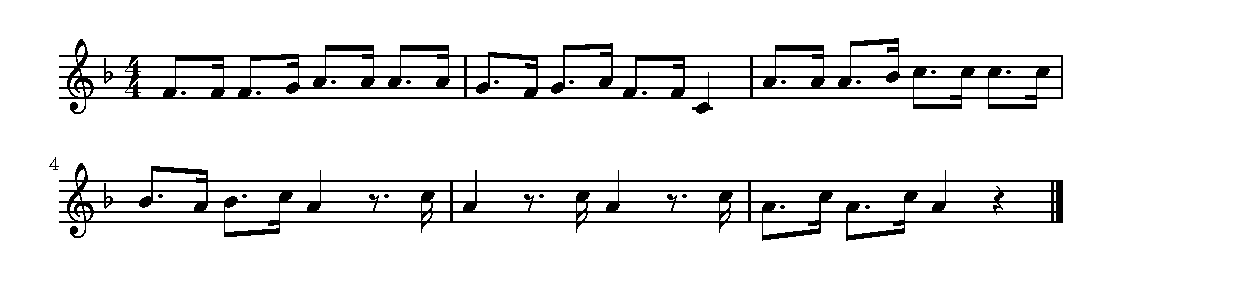
\includegraphics[clip]{shizukanakohan_crop.pdf}

\vspace{-10mm} \hspace{10mm}
静かな湖畔(しずかなこはんのもりのかげから)
\index{しずか@静かな湖畔(しずかなこはんのもりのかげから)}

\includegraphics[clip]{onnanomichi_crop.pdf}

\vspace{-10mm} \hspace{10mm}
女のみち(わたしがささげたそのひとに)
\index{おんな@女のみち(わたしがささげたそのひとに)}


\includegraphics[clip]{omochanochachacha_crop.pdf}

\vspace{-10mm} \hspace{10mm}
おもちゃのチャチャチャ
\index{おもちゃの@おもちゃのチャチャチャ}

\includegraphics[clip]{peergyntasagrieg_crop.pdf}

\vspace{-10mm} \hspace{10mm}
ペールギュントより朝(グリーグ)
\index{ぺーる@ペールギュントより朝(グリーグ)}

\includegraphics[clip]{hornmozart_crop.pdf}

\vspace{-10mm} \hspace{10mm}
ホルン協奏曲第1番(モーツァルト)
\index{ほるん@ホルン協奏曲第1番(モーツァルト)}

\includegraphics[clip]{ikenoame_crop.pdf}

\vspace{-10mm} \hspace{10mm}
池の雨(ヤマハ音楽教室幼児科メロディー暗唱曲)
\index{いけ@池の雨(ヤマハ音楽教室幼児科メロディー暗唱曲)}

\includegraphics[clip]{turkbeethoven_crop.pdf}

\vspace{-10mm} \hspace{10mm}
ベートーベンのトルコ行進曲
\index{べーと@ベートーベンのトルコ行進曲}
\index{とるこ@ベートーベンのトルコ行進曲}

\includegraphics[clip]{genkotsu_crop.pdf}

\vspace{-10mm} \hspace{10mm}
げんこつやまのたぬきさん
\index{げんこつやまの@げんこつやまのたぬきさん}

\includegraphics[clip]{seija_crop.pdf}

\vspace{-10mm} \hspace{10mm}
聖者が街にやってくる(聖者の行進))
\index{せいじゃ@聖者が街にやってくる(聖者の行進))}

\includegraphics[clip]{kogitsune_crop.pdf}

\vspace{-10mm} \hspace{10mm}
こぎつね(こぎつねこんこんやまのなか)
\index{こぎつね@こぎつね(こぎつねこんこんやまのなか)}

\includegraphics[clip]{londonbashi_crop.pdf}

\vspace{-10mm} \hspace{10mm}
ロンドン橋(ろんどんばしおちた)
\index{ろんどん@ロンドン橋(ろんどんばしおちた)}

\includegraphics[clip]{marysanno_crop.pdf}

\vspace{-10mm} \hspace{10mm}
メリーさんの羊(めりーさんのひつじ)
\index{めりー@メリーさんの羊(めりーさんのひつじ)}

\includegraphics[clip]{abrahamunoko_crop.pdf}

\vspace{-10mm} \hspace{10mm}
アブラハムの子(あぶらはむにはしちにんのこ)
\index{あぶらはむ@アブラハムの子(あぶらはむにはしちにんのこ)}

\includegraphics[clip]{chatsumi_crop.pdf}

\vspace{-10mm} \hspace{10mm}
茶摘(ちゃつみ。なつもちかづくはちじゅうはちや)
\index{@茶摘(ちゃつみ。なつもちかづくはちじゅうはちや)}

\includegraphics[clip]{okinafurudokei_crop.pdf}

\vspace{-10mm} \hspace{10mm}
大きな古時計(おおきなのっぽのふるどけい)
\index{おおきなふる@大きな古時計(おおきなのっぽのふるどけい)}

\includegraphics[clip]{takibi_crop.pdf}

\vspace{-10mm} \hspace{10mm}
たき火(かきねのかきねのまがりかど)
\index{たきび@たき火(かきねのかきねのまがりかど)}

\includegraphics[clip]{shikinouta_crop.pdf}

\vspace{-10mm} \hspace{10mm}
四季の歌(はるをあいするひとは)
\index{しきの@四季の歌(はるをあいするひとは)}

\includegraphics[clip]{katatsumuri_crop.pdf}

\vspace{-10mm} \hspace{10mm}
かたつむり(でんでんむしむし)
\index{かたつむり@かたつむり(でんでんむしむし)}

\includegraphics[clip]{hotarukoi_crop.pdf}

\vspace{-10mm} \hspace{10mm}
ほたるこい
\index{ほたるこい@ほたるこい}

\includegraphics[clip]{kagome_crop.pdf}

\vspace{-10mm} \hspace{10mm}
かごめかごめ(かごのなかのとりは)
\index{かごめ@かごめかごめ(かごのなかのとりは)}

\includegraphics[clip]{kaerunogassho_crop.pdf}

\vspace{-10mm} \hspace{10mm}
かえるの合唱(かえるのうたがきこえてくるよ)
\index{かえる@かえるの合唱(かえるのうたがきこえてくるよ)}

\includegraphics[clip]{yukainamakiba_crop.pdf}

\vspace{-10mm} \hspace{10mm}
ゆかいな牧場(いちろうさんのまきばでいーあいいーあいおー)
\index{ゆかいな@ゆかいな牧場(いちろうさんのまきばでいーあいいーあいおー)}

\includegraphics[clip]{bunbunbun_crop.pdf}

\vspace{-10mm} \hspace{10mm}
ぶんぶんぶん(ぶんぶんぶんはちがとぶ)
\index{ぶんぶんぶん@ぶんぶんぶん(ぶんぶんぶんはちがとぶ)}

\includegraphics[clip]{okinakuri_crop.pdf}

\vspace{-10mm} \hspace{10mm}
大きな栗の木の下で(おおきなくりのきのしたで)
\index{おおきなくり@大きな栗の木の下で(おおきなくりのきのしたで)}

\includegraphics[clip]{tonbono_crop.pdf}

\vspace{-10mm} \hspace{10mm}
とんぼのめがね
\index{とんぼの@とんぼのめがね}

\includegraphics[clip]{oshogatsu_crop.pdf}

\vspace{-10mm} \hspace{10mm}
お正月(もういくつねるとおしょうがつ)
\index{おしょうがつ@お正月(もういくつねるとおしょうがつ)}

\includegraphics[clip]{tewotata_crop.pdf}

\vspace{-10mm} \hspace{10mm}
手をたたきましょう
\index{てをたたき@手をたたきましょう}

\includegraphics[clip]{gaisen_crop.pdf}

\vspace{-10mm} \hspace{10mm}
凱旋行進曲(ヴェルディ。アイーダ)
\index{がいせん@凱旋行進曲(ヴェルディ。アイーダ)}

\includegraphics[clip]{obladi_crop.pdf}

\vspace{-10mm} \hspace{10mm}
Ob-La-Di, Ob-La-Da (ビートルズ)
\index{おぶらでぃ@Ob-La-Di, Ob-La-Da (ビートルズ)}

\includegraphics[clip]{carrythatweight_crop.pdf}

\vspace{-10mm} \hspace{10mm}
Carry That Weight (ビートルズ)
\index{きゃりーざっと@Carry That Weight (ビートルズ)}

\includegraphics[clip]{acrossuniverse_crop.pdf}

\vspace{-10mm} \hspace{10mm}
Across the Universe (ビートルズ)
\index{あくろす@Across the Universe (ビートルズ)}

\includegraphics[clip]{yurakucho_crop.pdf}

\vspace{-10mm} \hspace{10mm}
有楽町で逢いましょう(あなたをまてばあめがふる)
\index{ゆうらくちょう@有楽町で逢いましょう(あなたをまてばあめがふる)}

\includegraphics[clip]{cosmos_crop.pdf}

\vspace{-10mm} \hspace{10mm}
秋桜(うすべにのこすもすがあきのひの)
\index{こすもす@秋桜(うすべにのこすもすがあきのひの)}

\includegraphics[clip]{dango3kyodai_crop.pdf}

\vspace{-10mm} \hspace{10mm}
だんご3兄弟(くしにささってだんごだんご)
\index{だんごさん@だんご3兄弟(くしにささってだんごだんご)}

\includegraphics[clip]{chimchimcheree_crop.pdf}

\vspace{-10mm} \hspace{10mm}
チム・チム・チェリー(ちむちむにーちむちむにー)
\index{ちむちむちぇりー@チム・チム・チェリー(ちむちむにーちむちむにー)}

\includegraphics[clip]{tetsuwan_crop.pdf}

\vspace{-10mm} \hspace{10mm}
鉄腕アトム(そらをこえてららら)
\index{てつわんあとむ@鉄腕アトム(そらをこえてららら)}

\includegraphics[clip]{yogiriyo_crop.pdf}

\vspace{-10mm} \hspace{10mm}
夜霧よ今夜もありがとう(しのびあうこいをつつむよぎりよ)
\index{よぎりよ@夜霧よ今夜もありがとう(しのびあうこいをつつむよぎりよ)}


\includegraphics[clip]{hoshinonagareni_crop.pdf}

\vspace{-10mm} \hspace{10mm}
星の流れに(ほしのながれにみをうらなって)
\index{ほしのながれに@星の流れに(ほしのながれにみをうらなって)}



\includegraphics[clip]{ichigatsuichijitsu_crop.pdf}

\vspace{-10mm} \hspace{10mm}
一月一日(いちがついちじつ、としのはじめのためしとて)
\index{いちがつ@一月一日(いちがついちじつ、としのはじめのためしとて)}



\includegraphics[clip]{kakkou_crop.pdf}

\vspace{-10mm} \hspace{10mm}
かっこう
\index{かっこう}



\includegraphics[clip]{kirakira_crop.pdf}

\vspace{-10mm} \hspace{10mm}
きらきら星(きらきらぼし)
\index{きらきら@きらきら星(きらきらぼし)}



\includegraphics[clip]{koinobori_crop.pdf}

\vspace{-10mm} \hspace{10mm}
こいのぼり(やねよりたかい)
\index{こいのぼり(やねよりたかい)}



\includegraphics[clip]{konomichi_crop.pdf}

\vspace{-10mm} \hspace{10mm}
この道(このみちはいつかきたみち)
\index{このみち@この道(このみちはいつかきたみち)}



\includegraphics[clip]{konoyonohana_crop.pdf}

\vspace{-10mm} \hspace{10mm}
この世の花(このよのはな。あかくさくはなあおいはな)
\index{このよの@この世の花(このよのはな。あかくさくはなあおいはな)}



\includegraphics[clip]{mickeymousemarch_crop.pdf}

\vspace{-10mm} \hspace{10mm}
ミッキーマウス・マーチ(ぼくらのくらぶのりーだーは)
\index{みっきーまうす@ミッキーマウス・マーチ(ぼくらのくらぶのりーだーは)}


\includegraphics[clip]{mikan_crop.pdf}

\vspace{-10mm} \hspace{10mm}
みかんの花咲く丘(みかんのはながさいている)
\index{みかんの@みかんの花咲く丘(みかんのはながさいている)}



\includegraphics[clip]{momiji_crop.pdf}

\vspace{-10mm} \hspace{10mm}
もみじ(あきのゆうひにてるやま)
\index{もみじ(あきのゆうひにてるやま)}



\includegraphics[clip]{mushinokoe_crop.pdf}

\vspace{-10mm} \hspace{10mm}
虫の声(あれまつむしがないている)
\index{むしのこえ@虫の声(あれまつむしがないている)}



\includegraphics[clip]{musunde_crop.pdf}

\vspace{-10mm} \hspace{10mm}
むすんでひらいて(むすんでひらいててをうってむすんで)
\index{むすんでひらいて(むすんでひらいててをうってむすんで)}



\includegraphics[clip]{nangoku_crop.pdf}

\vspace{-10mm} \hspace{10mm}
南国土佐を後にして(なんごくとさをあとにして)
\index{なんごくとさ@南国土佐を後にして(なんごくとさをあとにして)}





\includegraphics[clip]{onetwojenkka_crop.pdf}

\vspace{-10mm} \hspace{10mm}
ワンツー・ジェンカ(おおきくくちあけて)
\index{わんつーじぇんか@ワンツー・ジェンカ(おおきくくちあけて)}


\includegraphics[clip]{saikai_crop.pdf}

\vspace{-10mm} \hspace{10mm}
再会(さいかい。あえなくなってはじめてしった)
\index{さいかい@再会(さいかい。あえなくなってはじめてしった)}



\includegraphics[clip]{sakura_crop.pdf}

\vspace{-10mm} \hspace{10mm}
さくらさくら
\index{さくらさくら}



\includegraphics[clip]{shuchou_crop.pdf}

\vspace{-10mm} \hspace{10mm}
酋長の娘(わたしのらばさん)
\index{しゅうちょう@酋長の娘(わたしのらばさん)}




\includegraphics[clip]{smallworld_crop.pdf}

\vspace{-10mm} \hspace{10mm}
小さな世界(ちいさなせかい、It's a small world、せかいじゅうどこだって)
\index{ちいさなせかい@小さな世界(ちいさなせかい、It's a small world、せかいじゅうどこだって)}



\includegraphics[clip]{takedanokomori_crop.pdf}

\vspace{-10mm} \hspace{10mm}
竹田の子もりうた(もりもいやがるぼんから)
\index{たけだのこもり@竹田の子もりうた(もりもいやがるぼんから)}



\includegraphics[clip]{tonakai_crop.pdf}

\vspace{-10mm} \hspace{10mm}
赤鼻のトナカイ(Rudolph the Red-Nosed Reindeer、あかはなのとなかい、まっかなおはなの)
\index{あかはなの@赤鼻のトナカイ(Rudolph the Red-Nosed Reindeer、あかはなのとなかい、まっかなおはなの)}






\includegraphics[clip]{gensou_crop.pdf}

\vspace{-10mm} \hspace{10mm}
幻想即興曲(ショパン)
\index{げんそうそっきょうきょく@幻想即興曲(ショパン)}

\includegraphics[clip]{kimigayo_crop.pdf}

\vspace{-10mm} \hspace{10mm}
君が代(きみがよはちよにやちよに)
\index{きみがよ@君が代(きみがよはちよにやちよに)}

\includegraphics[clip]{schubertkomori_crop.pdf}

\vspace{-10mm} \hspace{10mm}
シューベルトの子守歌(ねむれねむらははのむねに)
\index{しゅーべると@シューベルトの子守歌(ねむれねむらははのむねに)}
\index{こもりうた@シューベルトの子守歌(ねむれねむらははのむねに)}

\includegraphics[clip]{schubertnobara_crop.pdf}

\vspace{-10mm} \hspace{10mm}
シューベルトの野ばら(わらべはみたりのなかのばら)
\index{しゅーべるとののばら@シューベルトの野ばら(わらべはみたりのなかのばら)}

\includegraphics[clip]{yakyuken_crop.pdf}

\vspace{-10mm} \hspace{10mm}
野球拳(やきゅうけん。やきゅうするならこういうぐあいにしやしゃんせ)
\index{やきゅうけん@野球拳(やきゅうけん。やきゅうするならこういうぐあいにしやしゃんせ)}

\includegraphics[clip]{akaikutsu_crop.pdf}

\vspace{-10mm} \hspace{10mm}
赤い靴(あかいくつはいてたおんなのこ)
\index{あかいくつ@赤い靴(あかいくつはいてたおんなのこ)}

\includegraphics[clip]{akatonbo_crop.pdf}

\vspace{-10mm} \hspace{10mm}
赤とんぼ(ゆうやけこやけのあかとんぼ)
\index{あかとんぼ@赤とんぼ(ゆうやけこやけのあかとんぼ)}

\includegraphics[clip]{amaironokami_crop.pdf}

\vspace{-10mm} \hspace{10mm}
亜麻色の髪の乙女(ヴィレッジ・シンガーズ。あまいろのながいかみをかぜが)
\index{あまいろの@亜麻色の髪の乙女(あまいろのながいかみをかぜが)}

\includegraphics[clip]{anokowatare_crop.pdf}

\vspace{-10mm} \hspace{10mm}
あの子はたあれ(あのこはたあれたれでしょね)
\index{あのこは@あの子はたあれ(あのこはたあれたれでしょね)}

\includegraphics[clip]{aogeba_crop.pdf}

\vspace{-10mm} \hspace{10mm}
仰げば尊し(あおげばとうとしわがしのおん)
\index{あおげば@仰げば尊し(あおげばとうとしわがしのおん)}

\includegraphics[clip]{chouchou_crop.pdf}

\vspace{-10mm} \hspace{10mm}
ちょうちょう(ちょうちょうちょうちょうなのはにとまれ)
\index{ちょうちょう(ちょうちょうちょうちょうなのはにとまれ)}

\includegraphics[clip]{countryroad_crop.pdf}

\vspace{-10mm} \hspace{10mm}
カントリー・ロード(かんとりーろーど、このみち)
\index{かんとりー@カントリー・ロード(かんとりーろーど、このみち)}

\includegraphics[clip]{donguri_crop.pdf}

\vspace{-10mm} \hspace{10mm}
どんぐりころころ(どんぐりころころどんぶりこ)
\index{どんぐりころころ(どんぐりころころどんぶりこ)}

\includegraphics[clip]{fujisan_crop.pdf}

\vspace{-10mm} \hspace{10mm}
富士山(ふじさん。あたまをくものうえにだし)
\index{ふじさん@富士山(ふじさん。あたまをくものうえにだし)}

\includegraphics[clip]{harugakita_crop.pdf}

\vspace{-10mm} \hspace{10mm}
春が来た(はるがきた)
\index{はるがきた@春が来た(はるがきた)}

\includegraphics[clip]{harukaze_crop.pdf}

\vspace{-10mm} \hspace{10mm}
春風(ふけそよそよふけはるかぜよ)
\index{はるかぜ@春風(ふけそよそよふけはるかぜよ)}

\includegraphics[clip]{harunoogawa_crop.pdf}

\vspace{-10mm} \hspace{10mm}
春の小川(はるのおがわはさらさらながる)
\index{はるのおがわ@春の小川(はるのおがわはさらさらながる)}


\includegraphics[clip]{usagi_crop.pdf}

\vspace{-10mm} \hspace{10mm}
うさぎ(うさぎうさぎなにみてはねる)
\index{うさぎ(うさぎうさぎなにみてはねる)}

\includegraphics[clip]{warewaumi_crop.pdf}

\vspace{-10mm} \hspace{10mm}
われは海の子(われはうみのこしらなみの)
\index{われはうみのこ@われは海の子(われはうみのこしらなみの)}

\includegraphics[clip]{yashinomi_crop.pdf}

\vspace{-10mm} \hspace{10mm}
椰子の実(やしのみ。なもしらぬとおきしまより)
\index{やしのみ@椰子の実(やしのみ。なもしらぬとおきしまより)}

\includegraphics[clip]{yesterdayonce_crop.pdf}

\vspace{-10mm} \hspace{10mm}
イエスタデイ・ワンス・モア(カーペンターズ)
\index{いえすたでいわんす@イエスタデイ・ワンス・モア(カーペンターズ)}

\includegraphics[clip]{yuki100p_crop.pdf}

\vspace{-10mm} \hspace{10mm}
勇気100パーセント(がっかりしてめそめそしてどうしたんだい)
\index{ゆうきひゃくぱーせんと@勇気100パーセント(がっかりしてめそめそしてどうしたんだい)}

\includegraphics[clip]{yorokobi_crop.pdf}

\vspace{-10mm} \hspace{10mm}
喜びの歌(はれたるあおぞらただようくもよ)
\index{よろこびのうた@喜びの歌(はれたるあおぞらただようくもよ)}

\newpage
\printindex

\end{document}
